% !TeX encoding = UTF-8

% 载入 SJTUThesis 模版
\documentclass[type=bachelor,oneside]{sjtuthesis}
% 选项
%   type=[doctor|master|bachelor],     % 可选(默认:master),论文类型
%   zihao=[-4|5],                      % 可选(默认:-4),正文字号大小
%   lang=[zh|en|de|ja],                % 可选(默认:zh),论文的主要语言
%   review,                            % 可选(默认:关闭),盲审模式
%   [twoside|oneside],                 % 可选(默认:twoside),双页或单页边距模式
%   [openright|openany],               % 可选(默认:openright),奇数页或任意页开始新章
%   math-style=[ISO|TeX],              % 可选 (默认:ISO),数学符号样式
\usepackage[hidelinks]{hyperref}


% 论文基本配置,加载宏包等全局配置
% !TEX root = ./main.tex

\sjtusetup{
  %
  %******************************
  % 注意:
  %   1. 配置里面不要出现空行
  %   2. 不需要的配置信息可以删除
  %******************************
  %
  % 信息录入
  %
  info = {%
    %
    % 标题
    %
    zh / title           = {大规模随机化实验复杂设计统计学性质探索},
    en / title           = {Exploration of Statistical Properties in Complex Design of Large-Scale Randomized Experiments
},
    %
    % 标题页标题
    %   可使用“\\”命令手动控制换行
    %
    % zh / display-title   = {上海交通大学学位论文\\ \LaTeX{} 模板示例文档},
    % en / display-title   = {A Sample Document \\ for \LaTeX-based SJTU Thesis Template},
    %
    % 关键词
    %
    zh / keywords        = {随机对照试验,协变量平衡,重随机化,区组随机化,分层随机化},
    en / keywords        = {randomized controlled trials, covariate balance, rerandomization, block randomization, stratified randomization},
    %
    % 姓名
    %
    zh / author          = {黄彬彬},
    en / author          = {\textbf{Huang Binbin}},
    %
    % 指导教师
    %
    zh / supervisor      = {刘林},
    en / supervisor      = {\textbf{Liu Lin}},
    %
    % 副指导教师
    %
    % assoc-supervisor  = {某某教授},
    % assoc-supervisor* = {Prof. Uom Uom},
    %
    % 学号
    %
    id              = {520070910035},
    %
    % 学位
    %   本科生不需要填写
    %
    zh / degree          = {学士},
    en / degree          = {Master of Engineering},
    %
    % 专业
    %
    zh / major           = {统计学},
    en / major           = {Statistics},
    %
    % 所属院系
    %
    zh / department      = {数学科学学院},
    en / department      = {School of Mathematical Sciences},
    %
    % 答辩日期
    %   使用 ISO 格式 (yyyy-mm-dd);默认为当前时间
    %
     date                 = {2023-05},
    %
    % 标题页显示日期
    %   覆盖对应标题页的日期显示,原样输出
    %
     zh / display-date    = {2024 年 05 月},
    %
    % 资助基金
    %
    % zh / fund  = {
    %                {国家 973 项目 (No. 2025CB000000)},
    %                {国家自然科学基金 (No. 81120250000)},
    %              },
    % en / fund  = {
    %                {National Basic Research Program of China (Grant No. 2025CB000000)},
    %                {National Natural Science Foundation of China (Grant No. 81120250000)},
    %              },
  },
  %
  % 风格设置
  %
  style = {%
    %
    % 论文标题页 logo 颜色 (red/blue/black)
    %
    % title-logo-color = black,
  },
  %
  % 名称设置
  %
  name = {
    % bib             = {References},
    % ack             = {谢\hspace{\ccwd}辞},
    % achv            = {攻读学位期间完成的论文},
    digest={},
  },
}

% 使用 BibLaTeX 处理参考文献
%   biblatex-gb7714-2015 常用选项
%     gbnamefmt=lowercase     姓名大小写由输入信息确定
%     gbpub=false             禁用出版信息缺失处理
\usepackage[backend=biber,style=gb7714-2015]{biblatex}
% 文献表字体
% \renewcommand{\bibfont}{\zihao{5}\fixedlineskip{15.6bp}}
% 文献表条目间的间距
\setlength{\bibitemsep}{0pt}
% 导入参考文献数据库
\addbibresource{refs.bib}

% 脚注格式
\usepackage[perpage,bottom,hang]{footmisc}

% 定义图片文件目录与扩展名
\graphicspath{{figures/}}
\DeclareGraphicsExtensions{.pdf,.eps,.png,.jpg,.jpeg}

% 确定浮动对象的位置,可以使用 [H],强制将浮动对象放到这里(可能效果很差)
% \usepackage{float}

% 固定宽度的表格
% \usepackage{tabularx}

% 使用三线表:toprule,midrule,bottomrule。
\usepackage{booktabs}

% 表格中支持跨行
\usepackage{multirow}

% 表格中数字按小数点对齐
\usepackage{dcolumn}
\newcolumntype{d}[1]{D{.}{.}{#1}}

% 使用长表格
\usepackage{longtable}

% 附带脚注的表格
\usepackage{threeparttable}

% 附带脚注的长表格
\usepackage{threeparttablex}

% 算法环境宏包
\usepackage[ruled,vlined,linesnumbered]{algorithm2e}
% \usepackage{algorithm, algorithmicx, algpseudocode}

% 代码环境宏包
\usepackage{listings}
\lstdefinestyle{lstStyleCode}{%
  aboveskip         = \medskipamount,
  belowskip         = \medskipamount,
  basicstyle        = \ttfamily\zihao{6},
  commentstyle      = \slshape\color{black!60},
  stringstyle       = \color{green!40!black!100},
  keywordstyle      = \bfseries\color{blue!50!black},
  extendedchars     = false,
  upquote           = true,
  tabsize           = 2,
  showstringspaces  = false,
  xleftmargin       = 1em,
  xrightmargin      = 1em,
  breaklines        = false,
  framexleftmargin  = 1em,
  framexrightmargin = 1em,
  backgroundcolor   = \color{gray!10},
  columns           = flexible,
  keepspaces        = true,
  texcl             = true,
  mathescape        = true
}
\lstnewenvironment{codeblock}[1][]{%
  \lstset{style=lstStyleCode,#1}}{}

% 直立体数学符号
\providecommand{\dd}{\mathop{}\!\mathrm{d}}
\providecommand{\ee}{\mathrm{e}}
\providecommand{\ii}{\mathrm{i}}
\providecommand{\jj}{\mathrm{j}}
\usepackage{bbold}

% 国际单位制宏包
\usepackage{siunitx}

% 定理环境宏包
% \usepackage{ntheorem}
\usepackage{amsthm}

% 绘图宏包
\usepackage{tikz}
\usetikzlibrary{arrows.meta, shapes.geometric}

% 一些文档中用到的 logo
\usepackage{hologo}
\providecommand{\XeTeX}{\hologo{XeTeX}}
\providecommand{\BibLaTeX}{\textsc{Bib}\LaTeX}

% 借用 ltxdoc 里面的几个命令方便写文档
\DeclareRobustCommand\cs[1]{\texttt{\char`\\#1}}
\providecommand\pkg[1]{{\sffamily#1}}

% hyperref 宏包在最后调用
\usepackage{hyperref}

% E-mail
\providecommand{\email}[1]{\href{mailto:#1}{\urlstyle{tt}\nolinkurl{#1}}}


\begin{document}
\setlength{\baselineskip}{20pt}

%TC:ignore

% 标题页
\maketitle

% 原创性声明及使用授权书
\copyrightpage
% 插入外置原创性声明及使用授权书
% 此时必须在导言区使用 \usepackage{pdfpages}
% \copyrightpage[scans/sample-copyright.pdf]

% 前置部分
\frontmatter
{
\fancyhead[LE,RO]{}
{
\ctexset{chapter={afterskip=26bp}}
% 摘要
% !TEX root = ../main.tex

\begin{abstract}[zh]
\addcontentsline{toc}{chapter}{摘 \quad 要}
 本文通过理论分析和模拟实验,深入探讨了随机对照试验中的协变量平衡问题及其解决方案。文章首先指出,虽然随机化可以在实验组和对照组之间平衡协变量,但在实际实验中,协变量分组可能存在不平衡现象。为此,文章提出了重随机化的方法,并详细介绍了其执行过程和统计学性质。接着,文章阐述了A/A 测试、区组随机化和分层随机化的具体做法和注意事项,并通过模拟实验,对比了这些随机化实验复杂设计方法的表现。结果显示,这些方法都能保持对平均处理效应的估计的无偏性,且使用重随机化和分层随机化后,平均处理效应估计的方差有很大程度的下降。
\end{abstract}

{
\newfontface{\arial}{Arial}[Scale=0.94]
\ctexset{chapter/format+={\arial}}
\begin{abstract}[en]
\addcontentsline{toc}{chapter}{ABSTRACT}
This article delves into the issue of covariate balance in randomized controlled trials through theoretical analysis and simulation experiments. The paper begins by noting that although randomization can balance covariates between treatment groups, imbalances in covariate grouping may still occur in practical experiments. To address this, the paper proposes the method of rerandomization and provides a detailed account of its implementation process and statistical properties. Furthermore, the article elaborates on the specific practices and design considerations of A/A testing, block randomization, and stratified randomization, comparing the performance of these randomized experimental design methods through simulation experiments. The results indicate that these methods maintain the unbiasedness of the average treatment effect estimates, and the use of rerandomization and stratified randomization significantly reduces the variance of the estimated average treatment effect.

\end{abstract}
}
}

{
\ctexset{chapter={afterskip=26bp}}
\renewcommand{\cftchapfont}{\zihao{4}\bfseries}
\renewcommand{\cftsecfont}{\zihao{-4}}
\renewcommand{\cftsubsecfont}{\zihao{5}}
% 目录
\tableofcontents
}
}
% % 插图索引
% \listoffigures*
% % 表格索引
% \listoftables*
% % 算法索引
% \listofalgorithms*
% % 符号对照表
% \input{contents/nomenclature}

%TC:endignore

% 主体部分
\mainmatter

% 正文内容
{
\ctexset{chapter={afterskip=26bp}}
% !TEX root = ../main.tex

\chapter{绪论}

\section{引言}

第一次有记录的临床试验是由James Lind在1747年进行的,旨在找出治疗坏血病的方法\cite{dunn1997james}。经过百余年的发展,随机对照试验在医学、心理学、农业等领域都有着广泛的应用。到20世纪晚期,随机对照试验已经被认为是医学中“理性治疗”的标准方法\cite{meldrum2000brief}。随着技术进步,大规模数据的获取成为可能,随机对照试验在互联网行业大放异彩。在互联网行业中,大量新的交互方式、UI界面、推荐算法和新产品新功能的上线都会通过随机对照试验的验证。

由于随机化方法平衡了所有潜在的混杂因素,因而随机对照试验被视为估计因果效应的“金标准”,然而,如果在某个特定的实验中,随机化产生了在重要协变量上明显不平衡的分组结果。在这种情况下,我们需要回答一个重要的问题:如果我们观察到实验组和对照组在实验结果上的差异,那是来源于我们在实验中引入的处理因素,还是来源于分组后就预先存在的差异?

\section{本文研究主要内容}

针对上述问题,我们希望寻找相应的解决方案, 用以对分组之间的平衡程度进行检测,或是寻找使分组间相对更平衡的实验设计方案。A/A 测试、重随机化、区组随机化和分层随机化等随机化实验设计方法在一定程度上降低了不平衡分组产生的可能性。

本文将从三个部分展开,第一部分将从随机对照试验开始引入,并对重随机化的具体流程和统计学性质进行综述。第二部分着重于对A/A 测试、区组随机化和分层随机化的的具体做法和设计中的注意事项。最后一部分将结合数值实验,对比上述提到的随机化实验设计方法的表现。

\section{本文研究意义}

即使进行了随机化,实验组和对照组之间仍然可能存在差异的可能性比想象中的高。我们考虑每个受试者上的$d$个协变量,如性别、身高、体重等。假设$d$个协变量之间保持独立且设定显著性水平为$\alpha$,那么至少有一个协变量在实验组和对照组之间显示出显著差异的概率为$1-(1-\alpha)^d$。例如,当我们设定$d=14$且显著性水平为5\%时,这个概率可以高达51\%。正如Fisher所说,“大多数实验者在进行随机分配时会震惊地发现,不同分组的分布之间有多么不均等。”\cite{fisher1992arrangement}
因此在随机化实验设计中,仅仅进行随机化往往是不足够的。随机化实验复杂设计在随机对照试验中存在极大的价值,它可以防止试验中对照组和实验组出现较大偏差,产生在除各组接受的干预之外的变量比较性较强的组。本文的目的是介绍随机化实验复杂设计方法,包括随机对照试验的概念和意义,并综述几种随机化实验设计方案,以帮助实验设计者和研究人员更好地设计他们的随机对照试验。


\section{本章小结}

本文主要探讨如何在随机对照试验中有效地平衡实验组和对照组之间的差异。本章首先回顾了随机对照试验的历史和重要性,然后讲述了本文研究的主要内容:如何通过A/A测试、重随机化、区组随机化和分层随机化等方法来降低组间不平衡的可能性;通过数值实验对比这些随机试验设计方法的效果。本文的研究意义在于,通过这项研究,科研人员和实验设计者能更好地进行他们的随机对照试验,得到更有效力的因果推断。

% \section{研究内容}

% 研究的内容和文章讲述顺序

% 本毕业设计将研究重随机化等复杂实验设计的统计学性质。在阅读了相关文献后,我提出了以下可以进行探索研究的课题内容:
% \begin{enumerate}
%     \item 从理论上对重随机化等复杂实验设计的统计学性质进行一定的探究.
%     \item 结合理论与数值模拟探索重随机化及其他非完全随机化的复杂设计在大规模随机化实验中的统计学性质
%     \item 结合数值实验探究并比较重随机化实验、完全随机化实验和完全平衡分组对大规模实验设计的影响
%     \item 对比不同的重随机化算法(利用不同的组间距离判断准则)在可接受随机化的比例等算法计算效率指标上的表现。
%     \item 在协变量高维或样本量较大的情况下探究重随机化面临的挑战和问题。
% \end{enumerate}

% 1 综述和归纳重随机化的基础理论和相关结论。
% 2 了解重随机化算法的评价指标和影响重随机化效果的因素。
% 3 代码复现重随机化算法并通过数值实验得到重随机化对统计分析的影响。
% 4 数值实验:重随机化实验、随机化实验和完全平衡的实验分组的比较,得出相关结论。


% 2.2 随机化分组的不均衡问题

% 2.3 重随机化和其他平衡方法的文献回顾

% 2.4 研究缺口和贡献

% \section{研究意义}

% 重随机化的好处。。。文章提出了什么独特的点



% \section{本章小结}
% 本文……


% !TEX root = ../main.tex



\chapter{重随机化实验的流程设计及相关理论}\label{chap2}

\section{随机对照试验}

规模化的\textbf{随机对照试验}(Randomized Control Trial, RCT),也被称作 A/B testing, 被广泛应用于医学和技术领域。技术进步、在线交互和大规模数据的可获取性,使得科技公司能够将随机对照试验应用到大规模的在线实时数据中,通过数据驱动决策,加速了创新方案的实施和商业化的验证,极大地改进了用户体验并提升了公司收益\cite{kohavi2020online}。

在随机对照试验中,我们通常将模型中关注的、希望通过一定手段改变的核心指标(如医学实验中的死亡率,互联网行业中的点击率)称为实验的\textbf{结果变量}(Outcome Variable)或者\textbf{响应}(Responses), 其余变量则称为\textbf{协变量}(Covariates)或者\textbf{解释变量}(Explanatory Variables)。通常,人们感兴趣的研究为一个或多个协变量与响应的关联,因此必须要控制其余非主要感兴趣的协变量。我们将感兴趣的协变量也称作\textbf{处理变量}(Treatment Variables),如治疗方案、疾病类型、推荐算法等。

除了模型中包含的变量之外,其他变量也可能影响实验结果,例如仪器测试误差和环境变化等等。显然,我们无法控制所有可能影响响应的变量。从本质上讲,未观察到的变量不能包含在模型中,因为它们没有被观察到,而且在模型中包含太多的变量会降低实验的有效性。随机对照试验通过大量样本结合随机化的方法,在很大程度上防止了未观察到的变量的不当影响。

随机对照试验通常将提出的新方法与现有的方案进行比较,两组方案分别被称为“\textbf{实验}(Treatment)”和“\textbf{对照}(Control)”。当没有这样广泛接受的现行的处理方法可用时,需要在对照中使用\textbf{安慰剂}(Placebo),在对照组中采用这种处理方案的随机对照试验也被称为\textbf{盲法试验}(Blind Trial)。盲法试验可以避免实验设计者在评价实验结果时的主观因素、偏倚和安慰剂效应,以便获得更可靠的实验数据\cite{moher2010consort}。

\subsection{随机对照试验的流程}

随机对照试验的基本方法是,将收集到的研究对象随机分组,对不同组实施不同的干预,并对照实验结果的不同。在研究对象数量足够的情况下,这种方法可以有效地抵消已知和未知的混杂因素对各组实验的影响\cite{beller2002randomisation}。一般而言,随机对照试验的流程如下:

\begin{enumerate}
    \item 收集协变量数据;
    \item 将受试者\textbf{随机}分配到实验组和对照组;
    \item 根据步骤2中的随机分组结果分别进行实验;
    \item 分析实验结果。
\end{enumerate}

\subsection{随机对照试验的数学化表述\cite{morgan2012rerandomization}}
为了更好地从数学上说明随机对照试验的结论,本文会采用以下符号对随机对照试验做出定量化的表述。令 $\mathbf{X}$ 为 $n \times d$ 的协变量矩阵:
\begin{equation}
    \mathbf{X} = 
    \begin{bmatrix}
    \mathbf{x}_{1}^{\top} \\
    \mathbf{x}_{2}^{\top} \\
    \vdots \\
    \mathbf{x}_{n}^{\top}  
    \end{bmatrix}
    =
    \begin{bmatrix}
    x_{11} & x_{12} & \cdots & x_{1d} \\
    x_{21} & x_{22} & \cdots & x_{2d} \\
    \vdots & \vdots & \ddots & \vdots \\
    x_{n1} & x_{n2} & \cdots & x_{nd} 
    \end{bmatrix}.
\end{equation}


它表示在 $n$ 个受试者(样本)上测量的 $d$ 个维度的协变量。这里我们假定$\mathbf{X}$是已经被抽样后选定的固定的受试者。此处我们并未考虑从所有样本中抽取$n$个受试者的抽样机制,我们只关心在这个随机对照试验中获得的因果效应估计对于选定受试者$\mathbf{X}$中真实因果效应的估计准确度如何。除此之外,我们令$n$维$0-1$向量$\mathbf{W}=(w_1, w_2, \cdots, w_n)^{\top}$表示$n$个受试者的分组分配结果(为了更加直接地展示结果,我们只考虑两种分组结果,即实验组和对照组,并在后文中将保持一致):
\begin{equation}
    w_i= \begin{cases}1, & \text { 如果}\mathbf{x}_i\text{被分到\textbf{实验组} }, \\ 0, &  \text { 如果}\mathbf{x}_i\text {被分到\textbf{对照组}. }\end{cases}
\end{equation}



根据受试者的分组分配结果$\mathbf{W}$进行实验,对分配到实验组的受试者施加相应的实验影响,对照组则施加安慰剂或现行的处理方案,我们可以得到实验结果$\mathbf{Y}=(y_1, y_2, \cdots, y_n)^{\top}$。 由于实验结果$\mathbf{Y}$可能会与分组结果$\mathbf{W}$相关,我们定义$y_i(w_i)$为第$i$个受试者在分组$w_i$下的实验结果,其中$i=1, 2, \cdots, n$。在随机对照试验的步骤4中,我们重点关注分组结果$\mathbf{W}$对实验结果$\mathbf{Y}$的影响。定义 $\mathbf{Y}_{o b s(\mathbf{W})}=(y_{obs, 1}, y_{obs, 2}, \cdots, y_{obs, n})^{\top}$ 为观察到的试验结果的向量,其中
\begin{equation}
    y_{obs, i}=y_i(1) w_i+y_i(0)\left(1-w_i\right).
\end{equation}


为了符号的简洁性,下标$obs$代替了$obs(\mathbf{W})$。如果假设对于任何受试者$\mathbf{x_i}$,新的处理方案并没有优越性,便可以得到$y_i(1) = y_i(0)$,也即对于任何分组结果$\mathbf{W}$,$\mathbf{Y}_{obs}$都是相同的。反之,若想要证明施加的新实验方案的有效性,我们需要说明实验结果$Y$在不同分组情况下具有差异性。
% 因此,固定Yobs并模拟许多可以接受的随机分配W,如果零假设为真,我们可以实证地创建任何估计量g(x,W,yobs)的分布。为了解释重新随机化,每个模拟的随机化也必须满足ϕ(x,W) = 1。一旦模拟的随机化达到了期望的数量,模拟随机化中估计的治疗效果与实验中观察到的极端或更极端的比例就是p值。尽管一个完全的置换测试(包括所有可接受的随机化)是得到精确p值的必要条件,但可以增加模拟随机化的数量,以提供任何期望级别的精确p值。这个测试可以包含任何用过的重新随机化程序,将保持测试的显著性水平[Moulton (2004)],适用于任何估计量。Brillinger,Jones 和 Tukey (1978), Tukey (1993)以及Rosenberger 和 Lachin [(2002), Chapter 7]都建议在使用受限随机化方案时使用随机化测试来评估显著性。
\subsection{平均处理效应ATE及其估计}

为了比较不同实验干预在随机对照试验中的效果,衡量实验组和对照组之间平均结果的差异,我们引入了\textbf{平均处理效应}(Average Treatment Effect, ATE)\cite{doi:10.1080/01621459.1986.10478354}, 它的定义如下:
\begin{equation}\label{Average Treatment Effect}
\begin{aligned}
\tau & \equiv \overline{\mathbf{Y}(1)}-\overline{\mathbf{Y}(0)} \\
& =\frac{\sum _{i=1}^n y_i(1)}{n}-\frac{\sum _{i=1}^n y_i(0)}{n} \\
& = \frac{1}{n}\sum _{i=1}^n\left(y_i(1)-y_i(0)\right).
\end{aligned}
\end{equation}

然而因为每个受试者无法同时位于实验组和对照组,我们无法在同一受试者$\mathbf{x}_i$身上同时观察到
$y_i(1)$ 和 $y_i(0)$。例如,在一个随机对照实验中,我们只能在被分配到实验组的受试者身上观察到$y_i(1)$,在对照组的受试者身上观察到
$y_i(0)$。在因果推断中,我们仅能观察到每个受试者的$y_i(w_i)$,而不能直接计算(\ref{Average Treatment Effect})中的$\tau$,所以我们仅能使用$\mathbf{Y}_{obs}$来估计$\tau$。为了得到进一步的结果,我们遵从Rubin的\textbf{稳定个体干预值假设}(The Stable Unit Treatment Value Assumption, \textbf{SUTVA})\cite{rubin1980randomization}, 简称\textbf{稳定性假设}:
\begin{enumerate}
    \item 当每一个受试者$\mathbf{x}_i$在确定分组结果$w_i$之后,潜在实验结果$y_i(w_i)$是固定不变的,不会随着其他受试者的分组变化而变化。这也就是说,受试者在不同的分组下没有交互作用;
    \item 实验干预对所有受试者都是相同的。
\end{enumerate}

在上述假设的基础上,我们一般使用实验组和对照组实验结果的样本均值的差值来估计平均处理效应$\tau$:
\begin{equation}\label{equ:ATE's ets}
    \hat{\tau} \equiv \bar{\mathbf{Y}}_{o b s, T}-\bar{\mathbf{Y}}_{o b s, C},
\end{equation}

其中
$$
\bar{\mathbf{Y}}_{o b s, T} \equiv \frac{\sum _{i=1}^n w_i y_i(1)}{\sum _{i=1}^n w_i} \quad \text { 且 } \quad \bar{\mathbf{Y}}_{o b s, C} \equiv \frac{\sum _{i=1}^n\left(1-w_i\right) y_i(0)}{\sum _{i=1}^n\left(1-w_i\right)} \text {. }
$$


\section{重随机化}

尽管被视为检验因果效应“金标准(gold standard)”的随机对照试验,使用随机化的方法,对所有潜在的混淆因素进行了平衡,然而如果在特定的随机对照试验中,随机化产生的组别在重要的协变量上出现了明显不平衡的现象,此次随机对照试验的因果推断的效力也必定会大打折扣。在这种情况下,不常见的做法是手动调整分组结果,或者简单地“随机化直到看起来不错”。这两种方法的可重复性都很差,并且可能引入意外的偏差。为了解决以上问题,重随机化的实验设计方法被统计学家提出。重随机化实现了对受试者分组不平衡现象的检验并重新分组,使得实验随机分组的结果保留了随机性和无偏性的同时,在一定指标下更加平衡,从而在一定程度上避免了随机分组的偶然性。本章接下来的这一部分会着重介绍重随机化的实验设计流程及相关理论结论。

\subsection{重随机化的流程}

\begin{figure}[!hbtp]
    \centering
    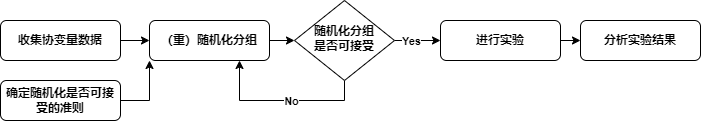
\includegraphics[width=1\linewidth]{figures/重随机化流程.png}
    \caption{重随机化的流程图}
    \label{fig:procedure of rerandomization}
\end{figure}

图\ref{fig:procedure of rerandomization}直观地展示了实施重随机化的流程。重随机化实验设计包含以下这些步骤:
\begin{enumerate}
    \item 收集协变量数据;
    \item 确定一个平衡标准,当随机化满足这个标准时,接受此次随机化;
    \item 将样本\textbf{随机}分配到实验组和对照组;
    \item 检查是否满足平衡标准:如果满足该标准,则前往步骤5;否则,返回步骤3;
    \item 根据步骤3中的随机分组结果分别进行实验;
    \item 分析实验结果。
\end{enumerate}

\subsection{重随机化的接受准则$\varphi$}\label{重随机化的接受准则}

根据图\ref{fig:procedure of rerandomization},在重随机化的流程中,我们需要预先确定一个随机化是否可以接受的准则。我们用函数$\varphi$表示重随机化是否可以接受的准则(Rerandomization Criterion),它是一个基于$\mathbf{X}$和$\mathbf{W}$的行可交换的标量函数,定义如下:
\begin{equation}
\varphi(\mathbf{X}, \mathbf{W})= \begin{cases}1, & \text { 如果 } \mathbf{W} \text { 是可接受的随机化, } \\ 0, & \text { 如果 } \mathbf{W} \text { 不是可接受的随机化 }.\end{cases}
\end{equation}

函数$\varphi$可能会根据不同协变量的相对重要性、实验设计者所期望的协变量平衡程度以及可用的计算能力而变化,但是无论如何选取$\varphi$,它都需要在实验进行前指定。

更一般地,我们可以指定一个随机化接受准则函数的集合 $S = \{\varphi_s\}$。在第$s$次重随机化时,我们可以通过一定的策略从集合$S$中选取某个随机化接受准则函数$\varphi_s$, 这种选取策略可以是确定的,也可以是随机的。例如类似于随机优化方法,在第$s$次随机化时并没有随机化出足够平衡的分组结果$\mathbf{W}$,我们可以在下一次随机化时选取更加宽容的随机化接受准则函数$\varphi_{s+1}$。因此,第$s$步的随机化接受准则函数可以表示为$\varphi_s(\mathbf{X}, \mathbf{W})$。但是在本文中,我们仅讨论所有随机化采用同一个接受准则函数的情况。

一旦我们提前确定随机化接受准则函数$\varphi$,且可接受的随机化的分组结果$\mathbf{W}$可以被枚举,那重随机化便等价于从预先确定的可接受随机化集合$\{\mathbf{W} | \varphi(\mathbf{X},\mathbf{W}) = 1\}$中随机选取分组结果$\mathbf{W}$\cite{kempthorne1955randomization}。但当可接受的随机化集合在事先难以枚举时,我们仍然要回到重随机化,在每次随机化后根据判定准则判断是否可以接受此次随机化分组的结果\cite{moulton2004covariate}。

从更广义上来说,重随机化是经典随机对照试验的推广。对于许多经典的实验设计,我们可以通过构造相应的函数$\varphi$对应到重随机化。例如,实验组和对照组所需要样本量相等的随机对照试验就等价于函数$\varphi(\mathbf{X}, \mathbf{W})= \begin{cases}1, & \sum _{i=1}^n w_i = \sum _{i=1}^n\left(1-w_i\right), \\ 0, & \sum _{i=1}^nw_i \neq \sum _{i=1}^n\left(1-w_i\right)\end{cases}$的重随机化试验。除此之外,我们也可以将重随机化和经典实验设计结合起来使用。重随机化相较于一些经典的实验设计如分层区组随机化等,它的优势是实验流程更加直接易懂。但是由于部分随机化生成的分组结果会被拒绝,因此生成一个可接受的随机化的时间往往会更长。

\subsection{可接受随机化的比例$P_a$}
% \subsection{the proportion of acceptable randomizations}

因为随机化实验的分析需要生成许多可接受的随机化,而重随机化生成每个可接受的随机化前可能会拒绝许多随机化生成的分组结果,由此可见,重随机化的计算时间是需要提前考虑的重要因素。为此,我们定义$P_a \equiv P(\varphi = 1)$为\textbf{可接受随机化的比例}(the Proportion of Acceptable Randomizations)。$P_a$的选择涉及到更平衡的随机化分组和计算时间之间的权衡:在计算性能相同时,较小的$P_a$可以确保实验组和对照组的协变量分配更加平衡,但也意味着获得一个可接受的随机化需要更长的平均等待时间。要获得一个可接受的随机化所需的随机化分组的次数遵循参数为$P_a$的几何分布,所以重随机化模拟$N$个可接受的随机化实验分组平均需要进行$\frac{N}{P_a}$次随机化分组。

所选的$P_a$必须留下足够的可接受的随机化分组结果来进行随机化实验。在小样本量的实验设计中,如果可接受随机化的准则设计得较为严苛,可能会出现满足可接受随机化准则的分组结果$\mathbf{W}$过少的现象从而导致分组失去随机性。实验设计者需要注意确保可接受的随机化分组的数量不会变得太小。如果在样本量足够大的实验设计中,上述问题一般不用考虑。这是因为,倘若某次要求实验组和对照组样本量相同的随机对照试验拥有$n$名受试者,随机分组结果的可能有$\binom{n}{n/2}$种。如果当$n=50$时,随机分组结果的数量的量级会达到$10^{14}$。


\section{重随机化的理论性质}

根据第\ref{重随机化的接受准则}节的描述,实验设计者可以根据需要选择任何可接受随机化准则函数$\varphi$,只要它是提前选定的。第\ref{无偏性}节描述了保持ATE的估计的无偏性所必需的条件。第\ref{马氏距离}节推荐了一类特定的函数,并研究了这种选择的统计学性质及其优劣势。
\subsection{保持ATE估计的无偏性}\label{无偏性}

\begin{theorem}\label{theorem 2.1}\cite{morgan2012rerandomization}
   若$\mathbf{W}$和$\mathbf{\varphi}$满足 $\sum _{i=1}^n w_i=\sum _{i=1}^n\left(1-w_i\right)$ 和$\varphi(\mathbf{X}, \mathbf{W})=\varphi(\mathbf{X}$, $\mathbf{1}-\mathbf{W})$,则 
   \begin{equation}
       \mathbb{E}(\hat{\tau} \mid \mathbf{X}, \varphi=1)=\tau.
   \end{equation} 
\end{theorem}

\begin{proof}

    若$\mathbf{W}$满足 $\sum _{i=1}^n w_i=\sum _{i=1}^n\left(1-w_i\right)$则有 $\sum _{i=1}^n w_i=\frac{n}{2}$。
    对于上述定理,我们有以下观察:$\mathbf{W}$和$1-\mathbf{W}$是可交换的。因此,在重随机化后,
    \begin{equation}
        \mathbb{E}(w_i \mid \mathbf{X}, \varphi=1)=\mathbb{E}(1-w_i \mid \mathbf{X}, \varphi=1)\  \forall i.
    \end{equation}
    
    因此,
    $$
        \begin{aligned}
        \mathbb{E}(\hat{\tau} \mid \mathbf{X}, \varphi=1) & =\mathbb{E}\left(\left.\frac{\sum_{i=1}^n w_i y_{i, o b s}}{\sum _{i=1}^n w_i}-\frac{\sum_{i=1}^n\left(1-w_i\right) y_{i, o b s}}{\sum _{i=1}^n (1-w_i)} \right\rvert\, \mathbf{X}, \varphi=1\right) \\
        & =\mathbb{E}\left(\left.\frac{\sum_{i=1}^n W_i y_i(1)}{n / 2}-\frac{\sum_{i=1}^n\left(1-w_i\right) y_i(0)}{n / 2} \right\rvert\, \mathbf{X}, \varphi=1\right) \\
        & =\frac{\sum_{i=1}^n \mathbb{E}\left(w_i \mid \mathbf{X},\varphi=1\right) y_i(1)}{n / 2}-\frac{\sum_{i=1}^n\left(1-\mathbb{E}\left(w_i \mid \mathbf{X}, \varphi=1\right)\right) y_i(0)}{n / 2} \\
        & =\frac{\sum_{i=1}^n(1 / 2) y_i(1)}{n / 2}-\frac{\sum_{i=1}^n(1 / 2) y_i(0)}{n / 2} \\
        & =\tau.
        \end{aligned}
    $$
\end{proof}

如果实验组和对照组分别被分到的受试者数量不同时,在重随机化后,$\hat{\tau}$不一定是$\tau$的无偏估计。我们可以给出以下反例:$\mathbf{X}=(2, 1, 0)^{\top}$, $\mathbf{Y}((1, 1, 1)^{\top}) = (0, 1, 1)^{\top}$ 且 $\mathbf{Y}((0, 0, 1)^{\top}) = (1, 0, 0)^{\top}$。同时,函数$\varphi(\mathbf{X}, \mathbf{W})= \begin{cases}1, & \frac{\sum_{i=1}^nw_i\mathbf{x}_i}{\sum_{i=1}^nw_i} = \frac{\sum _{i=1}^n\left(1-w_i\right)\mathbf{x}_i}{\sum _{i=1}^n\left(1-w_i\right)},\\ 0, & \frac{\sum _{i=1}^nw_i\mathbf{x}_i}{\sum _{i=1}^nw_i} \neq \frac{\sum _{i=1}^n\left(1-w_i\right)\mathbf{x}_i}{\sum _{i=1}^n\left(1-w_i\right)}.\end{cases}$
此函数定义的可接受随机化的准则用更直白的语言表述即是只接受两组均值差异为0的随机化分组。我们可以得到唯二可接受的随机化分组结果是$\mathbf{W}_1=(1, 0, 1)^{\top}$和$\mathbf{W}_2=(0, 1, 0)^{\top}$。但不论是$\mathbf{W}_1$还是$\mathbf{W}_2$,都有$\hat{\tau}= 1/2$ ,然而 $\tau = 1/3$,从而$\mathbb{E}(\hat{\tau} \mid \mathbf{x}, \varphi=1)\neq \tau$。



\subsection{使用 Mahalanobis 距离的重随机化}\label{马氏距离}

为了更方便地说明后续的理论结果,我们假定实验组和对照组的样本数量是提前确定的,且令$p_w$为实验组中样本数量占所有样本数量的比例,
\begin{equation}
    p_w=\frac{\sum_{i=1}^n w_i}{n}.
\end{equation}

令$d$维向量$\overline{\mathbf{X}}_T-\overline{\mathbf{X}}_C$表示实验组和对照组之间协变量的平均差值,
\begin{equation}\label{x_T-x_C}
    \overline{\mathbf{X}}_T-\overline{\mathbf{X}}_C=\frac{\mathbf{X}^{\top} \mathbf{W}}{n p_w}-\frac{\mathbf{X}^{\top}(\mathbf{1}-\mathbf{W})}{n\left(1-p_w\right)}=\frac{\mathbf{x}^{\top}\left(\mathbf{W}-p_w \mathbf{1}\right)}{n p_w\left(1-p_w\right)} .
\end{equation}

Mahalanobis 距离很好地衡量了两样本的组间距离,它的定义如下:

\begin{equation}\label{M's def}
    \begin{aligned}
        M & \equiv\left(\overline{\mathbf{X}}_T-\overline{\mathbf{X}}_C\right)^{\top}\left[\operatorname{cov}\left(\overline{\mathbf{X}}_T-\overline{\mathbf{X}}_C\right)\right]^{-1}\left(\overline{\mathbf{X}}_T-\overline{\mathbf{X}}_C\right) \\
        & =n p_w\left(1-p_w\right)\left(\overline{\mathbf{X}}_T-\overline{\mathbf{X}}_C\right)^{\top} \operatorname{cov}(\mathbf{X})^{-1}\left(\overline{\mathbf{X}}_T-\overline{\mathbf{X}}_C\right),
    \end{aligned}
\end{equation}

其中$\operatorname{cov}(\mathbf{X})$是$\mathbf{X}$的\textbf{样本协方差矩阵}(Sample Covariance Matrix)。$n, p_w$和$\operatorname{cov}(\mathbf{X})$都是已知的常数。此处,若$\operatorname{cov}(\mathbf{X})$为奇异矩阵(Singular Matrix),例如$d \geq n$, 应当使用$\operatorname{cov}(\mathbf{x})$的广义逆(Pseudo-inverse)替换掉$\operatorname{cov}(\mathbf{X})^{-1}$。

当某次随机化的$M$低于某个阈值$a$时,该次随机化被视为可接受的。令$P_a$为可接受的随机化所占的比例,因此
\begin{equation}
    P(M \leq a) = P_a,
\end{equation}
且重随机化的可接受准则函数$\varphi_{M}$为
\begin{equation}\label{重随机化准则}
    \varphi_{M}(\mathbf{X},\mathbf{W}) = \begin{cases}
        1,& \text{如果} M \leq a,\\
        0,& \text{如果} M > a.
    \end{cases}
\end{equation}

如果能得到$M$的分布,就能够指定$P_a$反解出需要的阈值$a$或是根据阈值$a$计算出$P_a$。如果不能直接得到$M$的分布,能够间接得到$M$的渐进分布,在样本量足够大的情况下也能实现以上效果。接下来,本文将说明关于$M$的分布的结论。

\subsubsection{$M$的渐进分布}
为了得到$M$的渐进分布的结果,我们需要以下两个引理。这两个引理我们不加证明直接给出。
\begin{lemma}\label{lemma:clt}\cite{erdos1959central}
 令 $\left\{a_n\right\}$ 为任意实数数列. 假设
$$
\begin{gathered}
M_n=\sum_{k=1}^n a_k, \\
D_n=\sqrt{\sum_{k=1}^n\left(a_k-\frac{M_n}{n}\right)^2},
\end{gathered}
$$
以及
$$
D_{n, s}=\sqrt{\frac{s}{n}\left(1-\frac{s}{n}\right)} D_n .
$$

定义 $N_{n, s}(x)$ 为不超过$\frac{s M_n}{n}+x D_{n, s}$的子列之和:
$$
a_{i_1}+a_{i_2}+\ldots+a_{i_8},\quad 1 \leqq i_1<i_2<\ldots<i_s \leqq n.
$$
定义以下函数
$$
F_{n, s}(x)=\frac{N_{n, s}(x)}{\binom{n}{s}} .
$$

令 $a_k^{\prime}=a_k-\frac{M_n}{n}$, 且
$$
d_{n, s}(\varepsilon)=\frac{1}{D_n^2} \sum_{\substack{\left|a_k\right|>D_n \\ 1 \leqq k \leq n}}\left|a_k^{\prime}\right|^2.
$$
如果 $n \rightarrow \infty, s=s_n \leq \frac{n}{2}$ 对任意 $\varepsilon>0$满足
$$
\lim _{n \rightarrow+\infty} d_{n, s_n}(\varepsilon)=0
$$
那么对于任何实数 $x$
$$
\lim _{n \rightarrow+\infty} F_{n, s_n}(x)=\Phi(x),
$$
其中$\Phi(x)$为标准正态分布的累计分布函数(cdf)。
    
\end{lemma}

\begin{lemma}\label{lemma:chisquare}\cite{mardia1979multivariate}
    若$\mathbf{Z} \sim \mathcal{N}_d(\mu, \Sigma)$,则$\mathbf{Z}^{\top}\left(\operatorname{cov}\mathbf{Z}\right)^{-1}\mathbf{Z} \sim \chi_d^2$。
\end{lemma}

\begin{theorem}\label{theorem:M's distribution}\cite{morgan2012rerandomization}
    $M \overset{d}\longrightarrow \chi_d^2$
\end{theorem}

\begin{proof}
    根据引理\ref{lemma:clt},$\overline{\mathbf{X}}_T-\overline{\mathbf{X}}_C$ 是渐近多元正态分布。如果$\overline{\mathbf{X}}_T-\overline{\mathbf{X}}_C$是多元正态分布,再由引理\ref{lemma:chisquare}并结合连续映射定理\cite{van2000asymptotic},我们可以得到定理\ref{theorem:M's distribution}中$M$的渐进分布结果。在此处证明中,需要注意的是,$\mathbf{X}$被视作固定不变的量,$M$的随机性来自于$\mathbf{W}$。
\end{proof}

我们可以使用数值模拟对$M$的渐进分布的结果进行验证。在下图中我们随机生成了$1000\times5$的$\mathbf{X}$,通过重复$10000$次$p_w = \frac{1}{2}$的随机分组,计算出$M$并绘制其频数直方图。通过和$\chi_5^2$的概率密度函数比较,我们可以发现两者吻合得很好。图\ref{fig:bisubcaptionbox}(b)中的Q-Q plot结果也很好印证了这一点。

\begin{figure}[!hbtp]
  \centering
  \subcaptionbox{$M$的频数直方图}%
                [7cm]{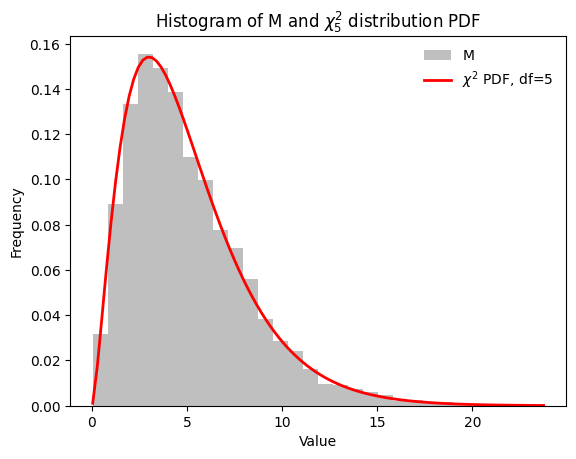
\includegraphics[height=6cm]{figures/chi-square.png}}
  \hspace{1cm}
  \subcaptionbox{$M$的Q-Q plot}%
                [7cm]{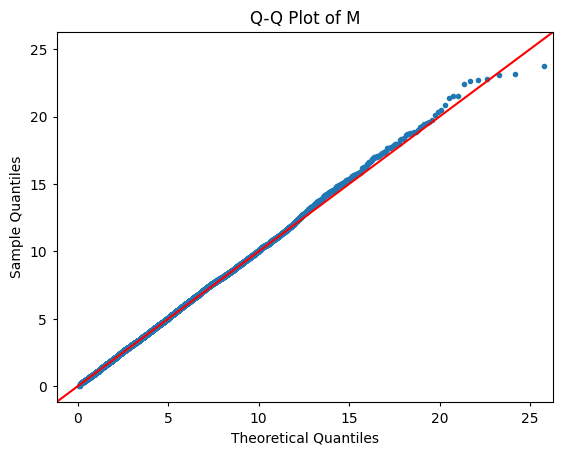
\includegraphics[height=6cm]{figures/qqplot.png}}
  \caption{$M$的渐进分布的数值模拟结果}
  \label{fig:bisubcaptionbox}
\end{figure}

如果样本量足够大,则我们可以提前指定$a$或$p_a$中的一个,然后利用定理\ref{theorem:M's distribution},$M \overset{d}\longrightarrow \chi^2_d$,求解出另一者。例如,在实际场景中,我们生成的$\mathbf{X}$的维数$d=5$,且要求重随机化的
可接受随机化的比例$P_a=80\%$,根据卡方分布的下80\%分位数结果得到$a=7.29$。

\subsubsection{平衡分组效应}

\begin{theorem}\label{theorem:covariance}\cite{morgan2012rerandomization}
    假定重随机化使用的准则为$\varphi_M$且$p_w=\frac{1}{2}$。若$\overline{\mathbf{X}}_T-\overline{\mathbf{X}}_C$服从多元正态分布,那么有
    \begin{equation}
        \operatorname{cov}\left(\overline{\mathbf{X}}_T-\overline{\mathbf{X}}_C \mid \mathbf{X}, \varphi_M=1\right)=v_a \operatorname{cov}\left(\overline{\mathbf{X}}_T-\overline{\mathbf{X}}_C \mid \mathbf{X}\right),
    \end{equation}
    其中
    \begin{equation}\label{def: va}
        v_a \equiv \frac{2}{d} \times \frac{\gamma(d / 2+1, a / 2)}{\gamma(d / 2, a / 2)}=\frac{P\left(\chi_{d+2}^2 \leq a\right)}{P\left(\chi_d^2 \leq a\right)}
    \end{equation}
    且 $\gamma$ 是不完全伽马函数(Incomplete Gamma Function): $\gamma(b, c) \equiv \int_0^c y^{b-1} e^{-y} d y$.
    
\end{theorem}

根据\ref{def: va}中$v_a$的定义,我们可以知道$0\leq v_a\leq 1$,再结合定理\ref{theorem:covariance}可以看出,重随机化减少了协变量均值差异的抽样方差,使得差异更加集中于0附近。我们定义\textbf{方差的百分比减少量}(the Percent Reduction in Variance),即重随机化减少每个协变量$\mathbf{x}_j$均值差异的方差的百分比:
\begin{equation}\label{varianceReduction}
100\left(\frac{\operatorname{var}\left(\bar{X}_{j, T}-\bar{X}_{j, C} \mid \mathbf{X}\right)-\operatorname{var}\left(\bar{X}_{j, T}-\bar{X}_{j, C} \mid \mathbf{X}, \varphi=1\right)}{\operatorname{var}\left(\bar{X}_{j, T}-\bar{X}_{j, C} \mid \mathbf{X}\right)}\right) .
\end{equation}

根据定理\ref{theorem:covariance}和定义\ref{varianceReduction},对于每个协变量,它的方差的百分比减少量为,
\begin{equation}
    100(1-v_a).
\end{equation}

\begin{figure}[!htbp]
    \centering
    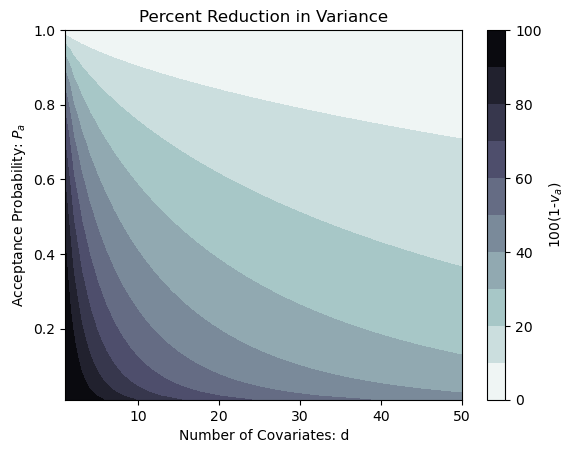
\includegraphics[width=0.55\linewidth]{figures/100(1-va).png}
    \caption{$\bar{X}_{T}-\bar{X}_{C}$的方差百分比减少量$100(1-v_a)$关于$d$和$P_a$的函数图像}
    \label{fig:100(1-va)}
\end{figure}

为了更加直观地展示方差的百分比减少量$100(1-v_a)$与协变量维数$d$和可接受随机化比例$P_a$的关系我们绘制了图\ref{fig:100(1-va)}。从图\ref{fig:100(1-va)}中我们可以发现,需要平衡的协变量维数$d$越小,可接受随机化比例$P_a$越接近0,协变量组间差异的均值的方差的百分比减少量$100(1-v_a)$越大。



\subsection{ATE的估计的准确性}

只要实验结果与协变量存在相关性,重随机化就能提高平均处理效应的估计$\hat{\tau}$的精度。因此,实验设计者可以仅仅以计算时间为代价,降低ATE的估计的方差,提升估计的准确性。

\begin{theorem}
    如果
    \begin{enumerate}
        \item 使用$\varphi_M$进行重随机化且$P_w=\frac{1}{2}$;
        \item 协变量$\mathbf{X}$和结果$\mathbf{Y}$均服从正态分布;
        \item 处理效应$\tau$是可加的,
    \end{enumerate}
    那么$\hat\tau$的方差的百分比减小量是
    \begin{equation}
        100(1-v_a)R^2,
    \end{equation}
    其中$R^2$表示在实验组内,结果$\mathbf{Y}$和协变量$\mathbf{X}$之间的多重相关系数的平方,而 $v_a$ 同定理\ref{theorem:covariance}中的定义一致。
\end{theorem}

\begin{figure}[!htbp]
    \centering
    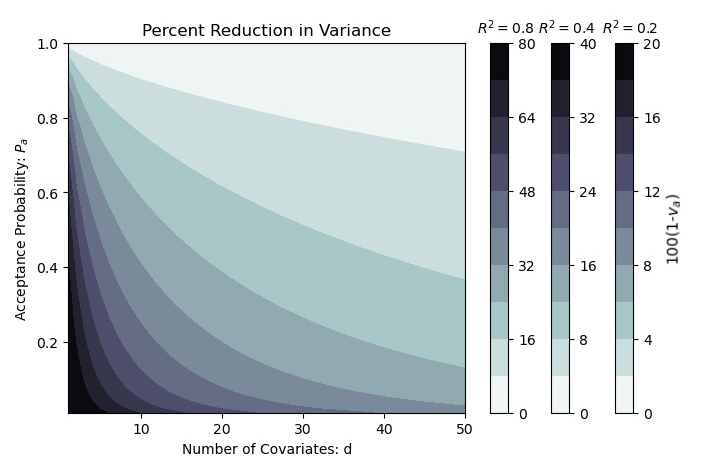
\includegraphics[width=0.68\linewidth]{figures/tau_percent_Reduction_in_Variance.png}
    \caption{$\hat\tau$的方差百分比减少量$100(1-v_a)$关于$d$、$P_a$和$R^2$的函数图像}
    \label{fig:tau_percent_Reduction_in_Variance}
\end{figure}

图\ref{fig:tau_percent_Reduction_in_Variance}所示的是平均处理效应的估计$\hat{\tau}$的方差百分比减少量关于$d$、$p_a$和$R^2$的函数图像。为了更好的可视化,此处选取了$R^2=0.8, 0.4, 0.2$,将$d$和$p_a$分别作为图像的横、纵坐标,绘制了图像。进一步地,我们可以发现,如果结果$\mathbf{Y}$和协变量$\mathbf{X}$之间的多重相关系数越大,平均处理效应的估计$\hat{\tau}$的方差百分比减少量越大。

\subsubsection{使用 Mahalanobis 距离的重随机化在高维数据下的挑战}

在统计学发展的大多数时间中,我们研究的每个样本上测量的特征数量相对较少,导致了传统理论和实践主要局限于“大样本量,小维数”的情形。近些年来,随着数据获取技术和计算设施的令人瞩目的发展,统计学研究的数据集中出现了许多数据量较少但是维度极大的情况,例如图像分析(image analysis),文本分类(document classification)与天文和大气科学等等\cite{johnstone2009statistical}。此时,许多传统的统计学习方法会面临维数灾难(Curse of Dimensionality)。使用 Mahalanobis 距离的重随机化也面临了高维数据的挑战,即如果$\mathbf{X}$的$\text{样本量}n <\text{维数}d$, 则使用可接受准则为$\varphi_M$的重随机化,无论如何选取分组结果$\mathbf{W}$,$M$都为确定的值。

我们对$100\times 200$的协变量矩阵$\mathbf{X}$进行了5000次随机平均分组,并计算了相应分组的Mahalanobis距离,进而绘制了Mahalanobis距离的频数直方图。如图\ref{fig:different Distance}(a)中对$M$的数值模拟结果所示,在高维的$\mathbf{X}$的情况下,准则$\varphi_M$会使得$M$失去随机性,从而导致重随机化失效。一旦设置好阈值$a$,无论如何选取$\mathbf{W}$, 重随机化只会一直接受或一直拒绝随机化分组。因此,在高维的场景下,实验设计者应当避免使用 Mahalanobis 距离参与重随机化。为此,实验设计者可以考虑使用欧氏距离即$\mathrm{l}_2$距离,类似于\ref{重随机化准则}构造相应的可接受随机化准则函数:
\begin{equation}
    D  \equiv\left(\overline{\mathbf{X}}_T-\overline{\mathbf{X}}_C\right)^{\top}\left(\overline{\mathbf{X}}_T-\overline{\mathbf{X}}_C\right). 
\end{equation}

\begin{figure}[!hbtp]
  \centering
  \subcaptionbox{$M$、$M_1$和$D$的频数直方图}%
                [7cm]{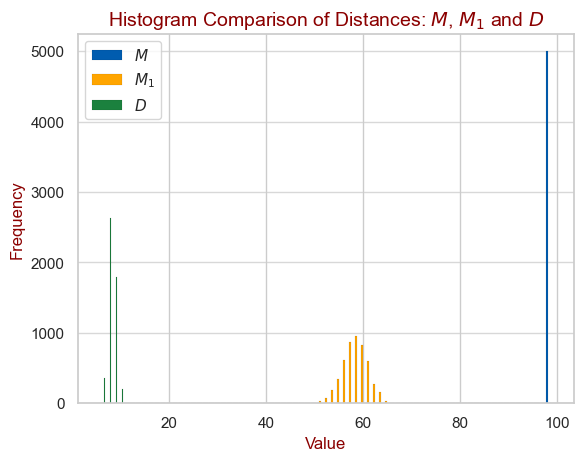
\includegraphics[height=6cm]{figures/differentDistance.png}}
  \hspace{1cm}
  \subcaptionbox{$M_{\lambda}$的均值和方差关于$\lambda$的折线图}%
                [7cm]{\includegraphics[height=6cm]{figures/Mahalanobis distance’s mean and variance.png}}
  \caption{$M$、$M_1$和$D$的数值模拟结果}
  \label{fig:different Distance}
\end{figure}

\begin{figure}[!htbp]
    \centering
    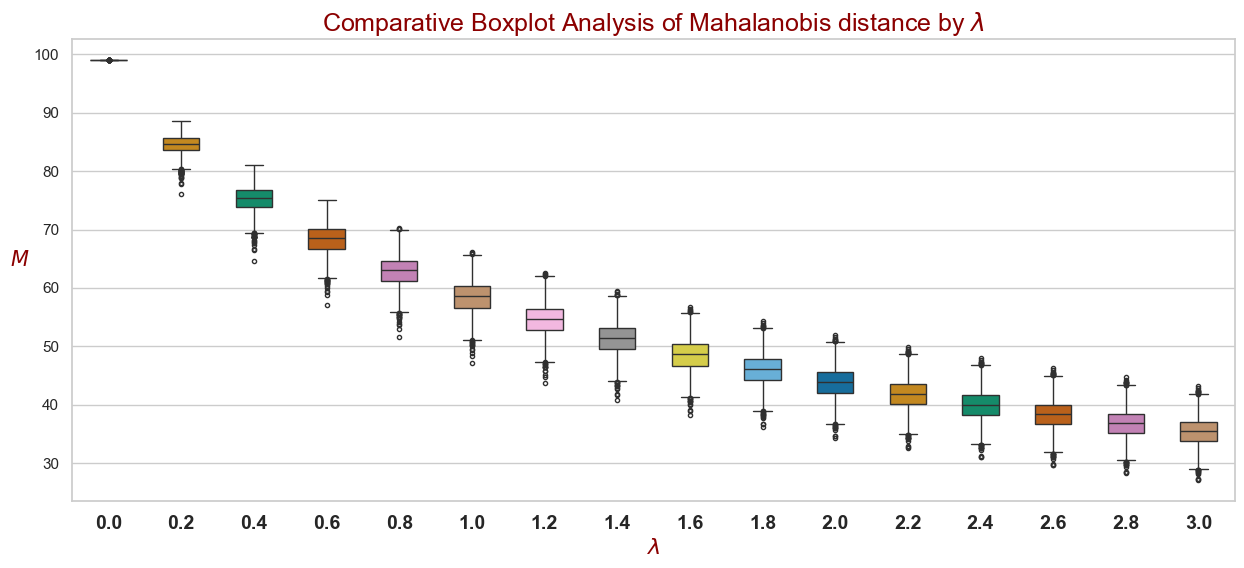
\includegraphics[width=1\linewidth]{figures/boxplot_Mahalanobis_distance_by_lambda.png}
    \caption{$M_{\lambda}$关于$\lambda$的箱线图}
    \label{fig:M_lambda's boxplot}
\end{figure}

或者,我们可以对使用Mahalanobis距离的可接受随机化函数进行一定的调整:加入正则化项$\lambda I_d$。在加入正则化项后的Mahalanobis距离具体表达式如下:
\begin{equation}
    M_{\lambda}=n p_w\left(1-p_w\right)\left(\overline{\mathbf{X}}_T-\overline{\mathbf{X}}_C\right)^{\top} \left(\operatorname{cov}(\mathbf{X})+\lambda I_d\right)^{-1}\left(\overline{\mathbf{X}}_T-\overline{\mathbf{X}}_C\right),\ \lambda > 0.
\end{equation}

如图\ref{fig:different Distance}(a)中$M_1$和$D$的频数直方图所示,无论是使用$\mathrm{l}_2$距离,还是对Mahalanobis距离加入正则化项,随着随机化产生了不同的分组结果$W$,组间距离都保持了随机性。从图\ref{fig:different Distance}(b)和图\ref{fig:M_lambda's boxplot}中可以看出,随着选取的$\lambda$的增大,随机化产生的$M_{\lambda}$的均值会减小。而$M_{\lambda}$的方差则呈现先上升后下降的趋势。由此可见,实验设计者应当避免选取过大的$\lambda$,以免出现$M_{\lambda}$的随机性不足的情况。

% \begin{theorem}\label{M's disadvantage}
%     假定重随机化使用的准则为$\varphi_M$且$P_w=\frac{1}{2}$。若对于$n\times d$的$\mathbf{x}$满足 $n < d$和$\operatorname{Rank}(\mathbf{x}) = n$,则对于任意分组$\mathbf{W}$, 有
%     $$
%     M \equiv \mathbb{1}_{T-C}^{\top}H^{-1}\mathbb{1}_{T-C}.
%     $$
%     其中,$\mathbb{1}_{T-C} = \mathbf{W} - (\mathbb{1} - \mathbf{W})$, $H = I_{n} - \frac{1}{n}\mathbb{1}_{n}\mathbb{1}_{n}^{\top}$。$\mathbb{1}_{n}$为$n$维全1列向量,$I_n$为$n\times n$的单位阵。
% \end{theorem}

% \begin{proof}
%     由定义\ref{x_T-x_C},
%     \begin{equation}
%         \overline{\mathbf{X}}_T-\overline{\mathbf{X}}_C=\frac{\mathbf{X}^{\top} \mathbf{W}}{n/2}-\frac{\mathbf{X}^{\top}(\mathbf{1}-\mathbf{W})}{n/2}=\frac{2}{n}\mathbf{X}^{\top}\mathbb{1}_{T-C} .
%     \end{equation}
%     根据定义\ref{M's def},
%     \begin{equation}\label{M in theorem 2.4}
%         \begin{aligned}
%             M & =n p_w\left(1-p_w\right)\left(\overline{\mathbf{X}}_T-\overline{\mathbf{X}}_C\right)^{\top} \operatorname{cov}(\mathbf{X})^{-1}\left(\overline{\mathbf{X}}_T-\overline{\mathbf{X}}_C\right)\\
%             & = \frac{1}{n}\mathbb{1}_{T-C}^{\top}\mathbf{X}\operatorname{cov}(\mathbf{X})^{-1}\mathbf{X}^{\top}\mathbb{1}_{T-C}.
%         \end{aligned}
%     \end{equation}
%     接下来关于样本均值$\bar{\mathbf{X}}$和样本方差$\operatorname{cov}(\mathbf{X})$做出一些推导,
%     \begin{equation}
%         \bar{\mathbf{X}} = \frac{1}{n}\sum_{i=1}^n \mathbf{X}_i = \frac{1}{n}\mathbf{X}^{\top}\mathbb{1}_n,
%     \end{equation}
%     \begin{equation}
%         HH^{\top} = (I_{n} - \frac{1}{n}\mathbb{1}_{n}\mathbb{1}_{n}^{\top})(I_{n} - \frac{1}{n}\mathbb{1}_{n}\mathbb{1}_{n}^{\top})^T = H,
%     \end{equation}
%     \begin{equation}\label{cov(X)}
%         \begin{aligned}
%              \operatorname{cov}(\mathbf{X})&=\frac{1}{n} \sum_{i=1}^n\left(\mathbf{x}_i-\bar{\mathbf{X}}\right)\left(\mathbf{x}_i-\bar{\mathbf{X}}\right)^T\\
%             &= \frac{1}{n}\left(\mathbf{x}_1-\bar{\mathbf{X}},\cdots, \mathbf{X}_n-\bar{\mathbf{X}}\right)\left(\mathbf{x}_1-\bar{\mathbf{x}},\cdots, \mathbf{x}_n-\bar{\mathbf{x}}\right)^T\\
%             &= \frac{1}{n} \left(\mathbf{X}^{\top} - \bar{\mathbf{X}}\mathbb{1}_{n}^{\top}\right)\left(\mathbf{X}^{\top} - \bar{\mathbf{X}}\mathbb{1}_{n}^{\top}\right)^{\top}\\
%             &= \frac{1}{n} \left(\mathbf{X}^{\top} - \mathbf{X}^{\top}\mathbb{1}_{n}\mathbb{1}_{n}^{\top}\right)\left(\mathbf{X}^{\top} - \mathbf{X}^{\top}\mathbb{1}_{n}\mathbb{1}_{n}^{\top}\right)^{\top}\\
%             & = \frac{1}{n}\mathbf{X}^{\top}(I_{n} - \frac{1}{n}\mathbb{1}_{n}\mathbb{1}_{n}^{\top})(I_{n} - \frac{1}{n}\mathbb{1}_{n}\mathbb{1}_{n}^{\top})^{\top}\mathbf{X}\\
%             & = \frac{1}{n}\mathbf{X}^{\top}HH^{T}\mathbf{X}\\
%             & = \frac{1}{n}\mathbf{X}^{\top}H\mathbf{X}.
%         \end{aligned}
%     \end{equation}
%     对$\mathbf{X}$进行SVD分解,
%         \begin{equation}\label{SVD}
%             \mathbf{X} = U \Sigma V^{\top},
%         \end{equation}
%     其中$U$为$n\times n$的矩阵,$\Sigma$为$n\times n$的对角矩阵,$V$为$n\times d$的矩阵。
    
%     由于$\operatorname{Rank}(\mathbf{X})=m$,$U$为正交矩阵,满足
%     \begin{equation}
%         U^{\top}U=UU^{\top}=I_n. 
%     \end{equation}
%     将\ref{SVD}代回\ref{cov(X)},
%     \begin{equation}\label{cov(X)_1}
%         \begin{aligned}
%             \operatorname{cov}(\mathbf{X}) &= \frac{1}{n}V \Sigma U^{\top} H U \Sigma V^{\top}.\\
%         \end{aligned}
%     \end{equation}
%     将\ref{SVD}和\ref{cov(X)_1}代回\ref{M in theorem 2.4},
%     \begin{equation}
%         \begin{aligned}
%             M &= \mathbb{1}_{T-C}^{\top}U \Sigma V^{\top}(V \Sigma U^{\top} H U \Sigma V^{\top})^{-1}V \Sigma U^{\top}\mathbb{1}_{T-C}\\
%             &= \mathbb{1}_{T-C}^{\top}H\mathbb{1}_{T-C}.\\
%         \end{aligned}
%     \end{equation}
%     由$\mathbb{1}_{T-C} = \mathbf{W} - (\mathbb{1} - \mathbf{W})=2\mathbf{W}-\mathbb{1}$,
%     \begin{equation}
%         \begin{aligned}
%             M &= \mathbb{1}_{T-C}^{\top}H\mathbb{1}_{T-C}\\
%             &= (2\mathbf{W}-\mathbb{1})^{\top}H(2\mathbf{W}-\mathbb{1})\\
%             &= 4\mathbf{W}^{\top}H\mathbf{W}-4\mathbf{W}^{\top}H\mathbb{1}+\mathbb{1}^{\top}H\mathbb{1}.
%         \end{aligned}
%     \end{equation}
%     $H$是对角线元素相同且除对角线外其余元素也相同的$n\times n$方阵,故$M$不会随着$\mathbf{W}$的变化而变化。
    
% \end{proof}

% 由\ref{M's disadvantage}可知,

% 论文正文是主体,一般由标题、文字叙述、图、表格和公式等部分构成 \cite{Yang1999}。一般可包括理论分析、计算方法、实验装置和测试方法,经过整理加工的实验结果分析和讨论,与理论计算结果的比较以及本研究方法与已有研究方法的比较等,因学科性质不同可有所变化。
% \par 论文内容一般应由十个主要部分组成,依次为:1.封面,2.中文摘要,3.英文摘要,4.目录,5.符号说明,6.论文正文,7.参考文献,8.附录,9.致谢,10.攻读学位期间发表的学术论文目录\cite{Yu2012}。
% \par 以上各部分独立为一部分,每部分应从新的一页开始,且纸质论文应装订在论文的右侧。


% \section{字数要求}
% \subsection{本科论文要求}
% 各学科和学院自定。理工科研究类论文一般不少于2万字,设计类一般不少于1.5万字;医科、文科类论文一般不少于1万字。

\section{本章小结}

随机化可以在组之间平衡协变量,但这只是平均意义上的,在任何一个实验中,协变量分组之间可能存在不平衡的现象。重随机化提供了一种简单直观的方法,以改善随机对照试验的协变量平衡。要执行重随机化,需要预先确定一个随机化是否可接受的准则。为了保证无偏性,这个规则需要保证实验组和对照组的受试者数量的均衡。本章证明了给定协变量矩阵,在大样本的情况下,实验组和对照组间的Mahalanobis距离服从自由度为协变量维数的卡方分布。如果采取的标准是每当Mahalanobis距离超过某个阈值时就重随机化,那么重随机化可以降低两组间均值差异的方差,且当协变量与结果相关时,重随机化会增加处理效应估计的精确度。在面临高维数据时,使用Mahalanobis距离的重随机化会失去随机性。为了解决以上问题,实验设计者可以考虑使用其他方式构造可接受随机化准则函数。

% !TEX root = ../main.tex

\chapter{其他随机化实验复杂设计简介}\label{chap3}

除了重随机化之外,产生随机分配序列$\mathbf{W}$的常见方法还有许多。根据不同的场景,不同的随机化实验设计要求,实验设计者往往要采用合适的随机分配方案,以求得更优的实验结果和更有效的因果推断。

\section{A/A 测试}\label{chap3:AAtest}
\textbf{A/A 测试}(A/A testing)和重随机化实现平衡分组的方法近似,它们都对实验组和对照组之间仍可能存在的差异进行了检验;A/A测试和A/B测试在实验设计流程上是相同的,唯一区别在于实验组和对照组的受试者接受相同的实验影响A(一般为安慰剂或广泛现行的方案),因而得名A/A 测试。如果分组是相对均衡的,测试组和对照组之间不应该有显著的预先存在的差异。因为在A/A测试中,零假设在设计上是正确的,所以当正态性和独立性假设成立,且使用显著性水平为0.05时,实验结果在统计上出现显著差异的概率应该是5\%左右。因此,如果A/A测试的结果显示出分组之间存在显著的不平衡,即A/A 测试“失败”时,实验设计者应当考虑谨慎对待后续A/B测试的结果,并根据不平衡的严重程度,选择忽略、统计调整或重新进行实验\cite{AAtest}。

在第\ref{chap:4}章的数值模拟的A/A测试部分,我们将对随机分组的协变量$\mathbf{X}$进行A/A测试,如果没有通过检验,则拒绝此次随机化并重新随机分组,直到随机化出通过A/A测试的分组结果$\mathbf{W}$,进一步计算ATE的估计。

% 因此由实验程序测量的差异反映了机会或偏见。因为在A/A测试中,零假设在设计上是正确的,所以当使用p值截断值为0.05时,每个度量的统计显著差异应该是5\%左右。我们可以轻松进行大量的A/A测试,当正态性或独立和i.i.d.假设(即独立和同分布的数据)被违反时,度量的A/A失败率会更高或更低。A/A测试也被用来确保治疗和对照用户之间的合理平衡。他们在识别偏见方面非常有效,尤其是那些在平台级别引入的偏见。例如,我们可以使用A/A测试来识别持续效应(或残留效应),其中之前的实验会影响对同一用户进行的后续实验

\section{区组随机化}
\textbf{区组随机化}或\textbf{块随机化}(Block Randomization)实验设计是一种随机化实验设计方法,它解决了简单随机化可能无法给实验组和对照组分配数量相等的受试者的问题。这种方法中,样本被分成若干个指定大小的\textbf{区组}(block),每个区组内的样本在处理之前都被认为是同质的。然后,在每个区组内,样本被随机分配给实验组和对照组\cite{mcentegart2014block},进而完成随机化的过程。

\begin{figure}[!hbtp]
  \centering
  \subcaptionbox{平均分组的区组随机化}%
                [7cm]{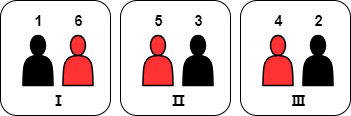
\includegraphics[height=2.2cm]{figures/blockRandom.drawio.png}}
  \hspace{1cm}
  \subcaptionbox{非平均分组的区组随机化}%
                [7cm]{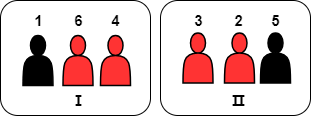
\includegraphics[height=2.25cm]{figures/blockRandom_inequal.drawio.png}}
  \caption{区组随机化的示意图}
  \label{fig:blockrandom}
\end{figure}

作为一个简单的例子,图\ref{fig:blockrandom}(a)说明了区组随机化的做法。它由三个含有两名受试者的区块组成:一名分配到实验组,有红色标出;一名分配到对照组,对应地由黑色标出。需要注意的是,区组内的分组顺序(先实验组还是先对照组)是对每个区块独立随机选择的。最后,将每个区组以随机的顺序组合在一起,得到最终的分组结果,这也是所有受试者进行实验的顺序。因此,区组随机化是从完全随机化的可能分组中的一个子集选取一个分组结果。区组随机化可以很好将顺序处理引入的偏差(例如测试仪器随着测试数量增加,误差会增大;药物疗效随批次变化可能有差异)尽可能地均匀分布在实验组和对照组中。同一个区组内的样本在处理顺序上是相邻的,且存在不同的实验处理,每一个区组内都很好地形成了一组对照。当认为需要防止响应随时间推移或批次变化而变化时,会使用区组随机化的设计,它保持了各个区组中的受试者始终相似。\cite{suresh2011overview}。

% 这种设计方式帮助研究人员控制不能或难以直接控制的顺序引入的潜在混杂因素,也有助于确保处理比例的均衡性。

值得注意的是,区组随机化也可以应对组间样本量不同的情况,只是在处理上略有不同。在第一步创建区组时,每个组的分配应当按照组间的比例进行。当实验组的数量为对照组的两倍时,如图\ref{fig:blockrandom}(b)所示,每个区组应当包含三名受试者,按照2:1的比例分配给实验组和对照组。其他组间数量的比例和更多组别的情况可以类似的处理。在设计区组随机化的过程中,需要注意的是,总样本量的大小应当能被区组大小整除\cite{burger2020importance}。


在第\ref{chap:4}章的数值模拟使用区组随机化时,我们将对协变量$\mathbf{X}$按照图\ref{fig:blockrandom}(a)的方式进行平均分组的区组随机化,进一步计算ATE的估计。



% 区组随机化是通过在块内随机化参与者来工作的,使得每种治疗都被分配了相等数量的参与者。例如,给定一个4个人的块,有6种可能的方式可以平等地将参与者分配到一个块。分配通过随机选择一个序列,并按照指定的顺序将下一个参与者块分配给研究组。注意,当总样本量大于可能排序的数量和块的大小的乘积时,可能会出现重复的块。此外,块大小必须能被研究组的数量整除。
% 块随机化的一个缺点是参与者的分配可能是可预测的,并且当研究组被揭示时可能会导致选择偏倚。也就是说,到目前为止在块中发生次数最少的治疗分配很可能会是下一个被选中的。通过使用随机块大小并保持调查者对每个块大小的盲目,可能会减少选择偏倚

\section{分层随机化}

\textbf{分层随机化}(Stratified Randomization)方法实现了控制和平衡协变量影响的需求。这种方法可以用来在一定程度上实现受试者在协变量上的组间平衡。研究者必须确定待平衡的协变量,并了解每个协变量对响应的潜在影响。对于每个受试者,根据其待平衡的协变量,分别进入相应所属的层。在所有受试者被识别并分配到相应的层次之后,在每个层内进行简单随机化,将受试者随机分配到实验组或者对照组。除此以外,分层随机化可以结合区组随机化一同使用,通过为协变量的每种组合生成一个单独的块,然后将受试者分配到相应的协变量块中,从而实现随机化。\cite{suresh2011overview}

\begin{figure}[!htbp]
    \centering
    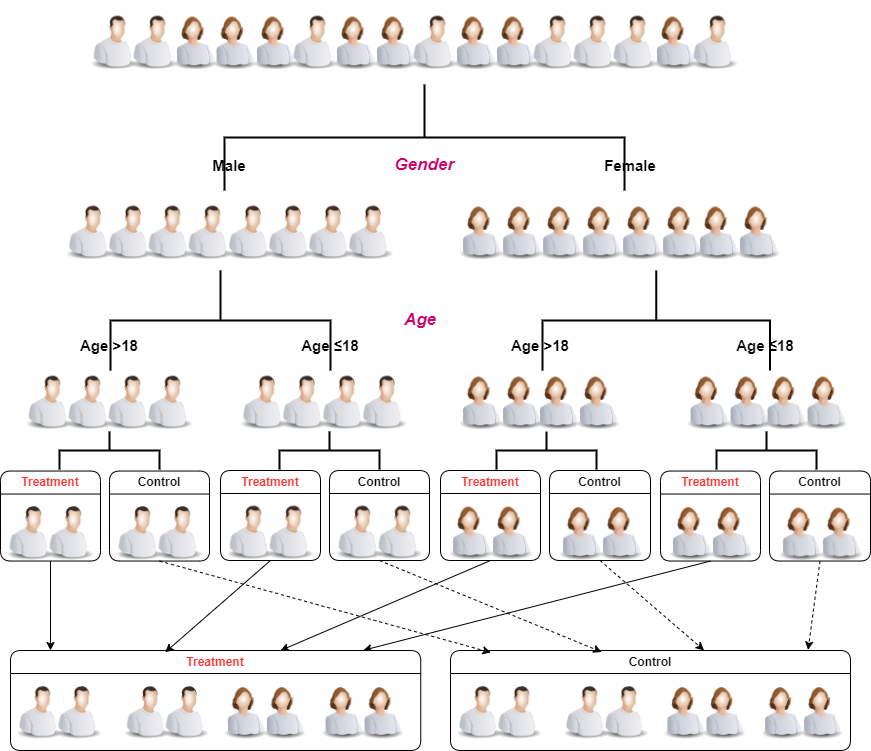
\includegraphics[width=0.8\linewidth]{figures/Stratified Randomization.drawio.png}
    \caption{分层随机化的示意图}
    \label{fig:Stratified Randomization}
\end{figure}

图\ref{fig:Stratified Randomization}展示了分层随机化的流程。实验设计者需要在研究前确定分层因素的水平,通过每个因素水平数的乘积得到总的层数。例如,在图\ref{fig:Stratified Randomization}中,我们想对受试者的性别和年龄进行分层,其中性别的水平数为2(男性和女性),年龄的水平数为2($\text{Age}>18$和$\text{Age} \leq 18$),进而计算出最终分出的层数为$2 \times 2=4$。对于每个受试者,根据其具体的性别和年龄,分别进入相应所属的层,再在每个层内独立随机进行实验分组。根据此方法,在性别和年龄这两个预先设置的协变量上,实验组和对照组的受试者保持了一定程度的平衡。

分层随机化常和区组随机化一同使用,它有助于确保层内的实验分配是平衡的。每个层都成为一个小试验,实验设计者可以认为层内的受试者在实验处理方面除外都是相似的,同一个层内的受试者被称为总体样本的一个亚组,研究者可以对亚组内的实验处理效应做出有效的推断\cite{kernan1999stratified}。例如,给定24名受试者,平均分为两个实验处理水平,安慰剂和治疗,以及两种性别,女性和男性。实验设计者可以考虑将24名受试者分为六组,每组四名受试者。四名受试者代表每种实验处理-性别组合(1:安慰剂女性,2:安慰剂男性,3:治疗女性,4:治疗男性)。随后,我们可以将每个组随机排序,得到最终的实验分组结果\cite{burger2020importance}。

分层随机化往往会使得分层因素在组间的分布相较于非分层的方案更平衡。当试验的总样本量较小(每个组别≤200名受试者)或计划进行涉及更大样本量的亚组分析时,可以考虑进行分层随机化。但是对于样本量非常大且不需要亚组分析(在某些因素上对照分析)的实验,通常不需要分层随机化,随机化分组基本上能实现实验组和对照组的平衡。除此之外,总的分层数应当保持克制,分层因素不宜过多,否则个别亚组内的受试者数量将很少甚至没有。建议分层的数量应当保持在$\frac{n}{B+4}$以下,其中$n$是总的样本大小,$B$为每个层内的样本数量\cite{kernan1999stratified}。

在第\ref{chap:4}章的数值模拟中使用区组随机化时,我们将对$n\times d$的协变量$\mathbf{X}$从$d$个因素中选取$k$个维度作为分层的因素进行分层随机化,其中每个维度的两个水平设置为大于等于和小于该因素的均值。平均而言,每个层内包含的样本量为$\frac{n}{2^k}$。由分层随机化的分组结果进一步计算ATE的估计。

\section{本章小结}
在本章中着重介绍了A/A 测试、区组随机化和分层随机化的具体做法和设计中的注意事项。A/A测试对实验组和对照组采用相同的实验影响,观察实验结果是否存在显著差异,以用于检验分组的均衡性,并以此为根据判断相应的A/B 测试的效应。区组随机化在样本分为指定大小的区组,并在区组内随机分组。区组随机化在组间样本量相同或不同时都能应用,且能够将顺序处理引入的偏差平衡。分层随机化根据设计者预先确定的分层因素,将受试者分为多个层,在每个层次内随机分组得到最终的分组结果,因此能够很好地平衡预先指定的分层因素在组间的分布。此外,本章还对第\ref{chap:4}章中数值模拟后的抽样分组方案做出了阐述。


% !TEX root = ../main.tex

\chapter{数值模拟和验证}\label{chap:4}

\section{数值模拟的模型设置}

为了从数值上说明随机化实验复杂设计的结果,我们采取以下\textbf{线性可加模型}模拟出实验结果$\mathbf{Y}$:
    \begin{equation}\label{linear Model}
        \textit{\textbf{Linear Model}}:\quad y_i (w_i) | \mathbf{x}_i = \beta_0 + \beta_1^{\top}\mathbf{x}_i+\tau w_i + \epsilon_i,
    \end{equation}
    其中$\epsilon_i \sim N(0,\ \sigma^2)$。

\begin{figure}[!htbp]
    \centering
    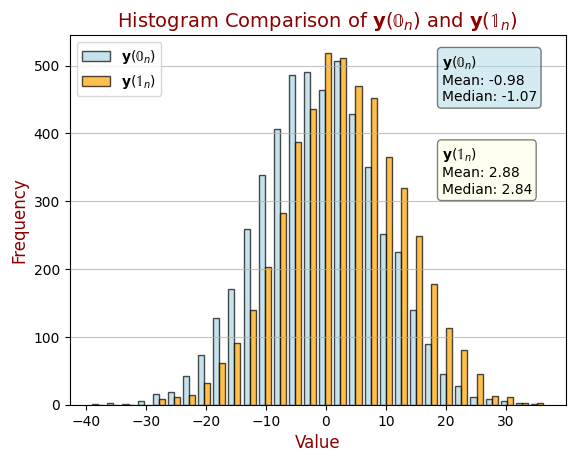
\includegraphics[width=0.75\linewidth]{figures/distributionOfy.png}
    \caption{$\mathbf{y}(\mathbb{0}_n)$和$\mathbf{y}(\mathbb{1}_n)$的频数直方图}
    \label{fig:distributionOfy}
\end{figure}

线性可加模型的参数$\beta_0$、$\beta_1$由均一分布随机抽取后标准化得到,而协变量$\mathbf{X}$从均值为$\mu_d$,方差为$\eta I_d$的多元正态分布中抽取。实验结果$y_i(0)=\beta_0 + \beta_1^{\top}\mathbf{x}_i+ \epsilon_i$和$y_i(1)=\beta_0 + \beta_1^{\top}\mathbf{x}_i+\tau + \epsilon_i$的频数直方图如\ref{fig:distributionOfy}所示。在图\ref{fig:distributionOfy}中,具体的参数设置为$n=5000, d=5, \tau=3, \mu_d = 0, \eta=1, \sigma^2=0.25$。图像中蓝色部分和黄色部分分别为将所有样本分配到对照组和实验组的结果:对于被分到对照组($w_i=0$)的样本$\mathbf{x}_i$,我们用蓝色标出;对于对于被分到实验组($w_i=1$)的样本$\mathbf{x}_i$,则选用黄色标出。在后续的随机化分组中,我们会选用固定的随机化出的协变量$\mathbf{X}$, 且为了形成有效的对照,所有随机化实验方案都使用相同的协变量$\mathbf{X}$。


\section{随机化方法与参数设置}
    我们将着重对重随机化、A/A 测试,区组随机化和分层随机化在代码上进行实现,并根据分组结果计算$\hat\tau$。为了避免偶然性,每种随机化方法都会重复10000次,并展示相应方法计算出的$\hat\tau$在均值和方差上的结果。具体每种随机化方法的设计如下。
    
\subsection{重随机化}
\begin{figure}[!htbp]
    \centering
    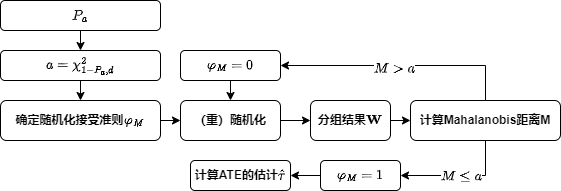
\includegraphics[width=0.8\linewidth]{figures/Rerandomization.drawio.png}
    \caption{重随机化实验设计的具体流程}
    \label{fig:RerandomizationDesign}
\end{figure}
此处我们采用可接受准则为$\varphi_M$的重随机化,为了平衡好计算时间与受试者在组间的分布差异,我们选取了$P_a=0.5$,进而可以求得相应的Mahalanobis距离的阈值$a=4.35$。具体实验设计流程如图\ref{fig:RerandomizationDesign}所示,理论上我们期望观察到重随机化后的$\hat{\tau}$在均值上应当和组间样本量相等的完全随机分组相近,但在方差上有所下降。

\begin{figure}[!htbp]
    \centering
    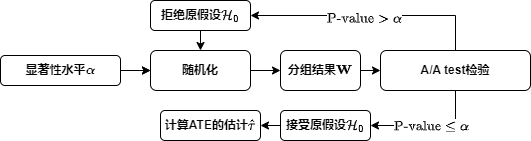
\includegraphics[width=0.8\linewidth]{figures/Chapter4AAtest.drawio.png}
    \caption{A/A test 实验设计的具体流程}
    \label{fig:AAtestDesign}
\end{figure}

\subsection{A/A 测试}

A/A 测试 的流程如图\ref{fig:AAtestDesign},和\ref{chap3:AAtest}中的阐述保持了一致。此处我们需要提前设置显著性水平$\alpha=0.05$, 也即是我们容许的组间存在显著差异的可能性为5\%。当分组结果$\mathbf{W}$没有通过A/A测试时,我们将拒绝此次分组结果并重新分组,直至出现通过A/A 测试的分组。

\subsection{区组随机化}
\begin{figure}[!htbp]
    \centering
    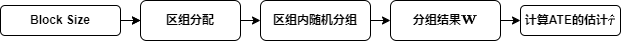
\includegraphics[width=0.8\linewidth]{figures/Chapter4Block.drawio.png}
    \caption{区组随机化实验设计的具体流程}
    \label{fig:BlockDesign}
\end{figure}

在进行如图\ref{fig:BlockDesign}的区组随机化之前我们需要设置每个区组的大小(Block Size),此处我们选取$\text{Block Size} = 2$,也即每个区组内部会有两名受试者分别被分到实验组和对照组。在医学实验中,受试者往往是逐一进入每个区组直至区组满员而进入下一个区组。但是我们预先生成了所有协变量$\mathbf{x}$,而每个样本之间没有先后次序之分,因此我们采取先将受试者随机分配至$n/2$个区组中,再在区组内进行二次随机分配的方案。可以预见的,此处的区组随机化后的分组结果并不会优于组间样本量相等的完全随机分组,这是由于我们并没有引入顺序影响的误差。


\subsection{分层随机化}
\begin{figure}[!htbp]
    \centering
    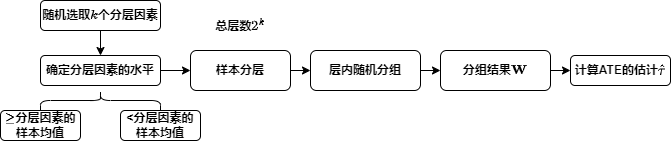
\includegraphics[width=0.8\linewidth]{figures/Chapter4Stratified.drawio.png}
    \caption{分层随机化实验设计的具体流程}
    \label{fig:StratifiedDesign}
\end{figure}

在进行分层随机化前,实验设计者需要确定对实验结果影响较大的混杂因素如性别、年龄等。在此处由于所有协变量$\mathbf{X}$由从正态分布中随机生成,因而不存在上述明确可以选择的分层因素。为此,我们采取随机选取$k=3$($k<d$)个维度作为分层因素,分层因素的水平人为设置为大于等于分层因素的样本均值和小于分层因素的样本均值。因而我们可以得到$2^k$个层。在此基础上,我们根据图\ref{fig:StratifiedDesign}中的流程,在样本的分层之后,在每个层次内部随机分组,进而得到最终的分组结果$\mathbf{W}$。

\section{随机化方法对$\hat{\tau}$的影响}
根据使用不同的随机化设计重复10000次实验分组之后,我们可以计算出5组$\hat{\tau}$。图\ref{fig:Comparative Boxplot Analysis}分别展示这5组$\hat{\tau}$的箱线图结果,红色虚线则标注出了真实的$\tau$的值。图\ref{tab:Comparative stats Analysis of Average Treatment Effects}则直接展示了5组平均处理效应的估计$\hat{\tau}$的均值和方差的结果。
\begin{figure}[!htbp]
    \centering
    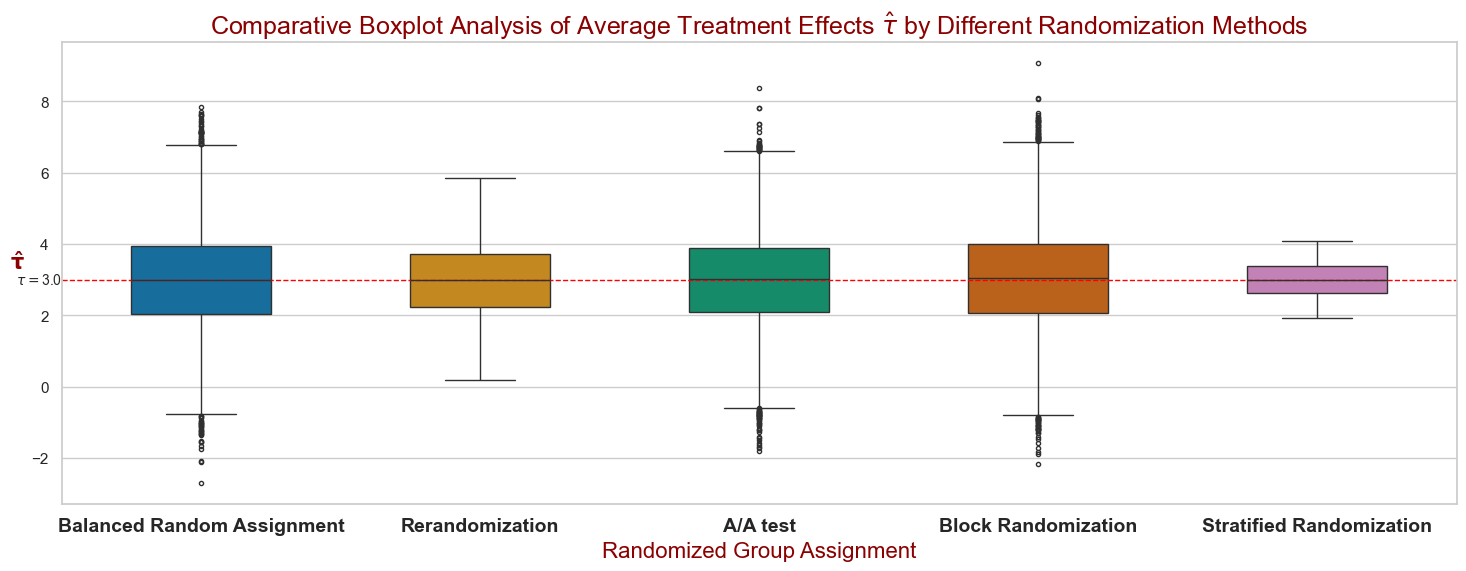
\includegraphics[width=1.00\linewidth]{figures/Comparative Boxplot Analysis of Average Treatment Effects.png}
    \caption{不同随机化方法下平均处理效应$\hat{\tau}$的比较性箱线图分析($\tau=3.0$)}
    \label{fig:Comparative Boxplot Analysis}
\end{figure}

\begin{table}[!htbp]
    \centering
        \begin{tabular}{lcc}
        \toprule
         & mean & variance \\
        \midrule
        Balanced Random Assignment & 3.00 & 1.98 \\
        Rerandomization & 2.99 & 1.04 \\
        A/A testing & 3.01 & 1.90 \\
        Block Randomization & 3.01 & 2.03 \\
        Stratified Randomization & 3.00 & 0.13 \\
        \bottomrule
        \end{tabular}
    \caption{不同随机化方法下平均处理效应的估计$\hat{\tau}$的统计结果($\tau=3.0$)}
    \label{tab:Comparative stats Analysis of Average Treatment Effects}
\end{table}

重随机化、A/A 测试、区组随机化、分层随机化都很好得保持了对$\tau$的估计的无偏性,且重随机化、分层随机化在$\hat{\tau}$的方差上有明显的下降,其中分层随机化在估计$\tau$的方差下降尤为明显,对$\tau$的估计更为精准。尽管重随机化在估计$\tau$的方差下降不如分层随机化,但是重随机化在计算时间上更为占优,它用相对于分层随机化更少的计算时间获得不错的方差下降。

\section{重随机化$P_a$对$\hat{\tau}$的影响}

\begin{figure}[ht]
    \centering
    \begin{minipage}{0.7\textwidth}
        \centering
        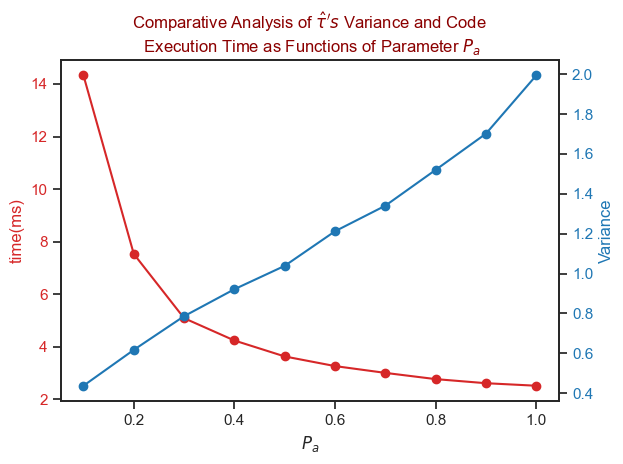
\includegraphics[width=\textwidth]{figures/重随机化Pa的影响.png} % 替换为实际的图片文件名
        \caption{不同$P_a$下$\hat{\tau}$的方差和平均重随机化时间($\tau=3.0$)}
       \label{fig:Comparative stats Analysis of Average Treatment Effects by Pa}
    \end{minipage}\hfill
    \begin{minipage}{0.3\textwidth}
        \centering
        \begin{tabular}{lcc}
            \hline
        $P_a$ & mean & variance \\
        \hline
            0.1 & 3.00 & 0.44 \\
            0.2 & 3.00 & 0.62 \\
            0.3 & 2.99 & 0.79 \\
            0.4 & 3.01 & 0.92 \\
            0.5 & 3.02 & 1.04 \\
            0.6 & 2.99 & 1.21 \\
            0.7 & 3.00 & 1.34 \\
            0.8 & 3.00 & 1.52 \\
            0.9 & 2.98 & 1.70 \\
            1.0 & 3.02 & 1.99 \\
            \hline
        \end{tabular}
        \caption{不同$P_a$下平均处理效应的估计$\hat{\tau}$的统计结果($\tau=3.0$)}
        \label{tab:Comparative stats Analysis of Average Treatment Effects by Pa}
    \end{minipage}
\end{figure}

对于不同的$P_a$,我们可以构造出不同的可接受随机化函数。在这一部分中,我们从0.1到1间隔为0.1选取了10个$P_a$,分别进行重随机化实验,得到了10组平均处理效应的估计$\hat{\tau}$。它们的均值和方差的结果如图\ref{tab:Comparative stats Analysis of Average Treatment Effects by Pa}所示。除此以外,对于不同的$P_a$,相应的平均重随机化耗时也被绘制在图\ref{fig:Comparative stats Analysis of Average Treatment Effects by Pa}中。从中我们可以发现,随着选取的$P_a$的增大,$\hat{\tau}$的方差也会逐渐增大,与此同时,平均的计算时间也会减小。在重随机化中,平均计算时间和估计的准确性不可兼得。采用重随机化时,实验设计者往往需要在平均处理效应的估计的准确性和平均计算时间中做好平衡。

\section{本章小结}
本章通过随机生成服从多元正态分布的协变量$\mathbf{X}$进而根据线性可加模型和分组结果模拟出实验结果$\mathbf{Y}$。接着本章阐述了不同随机化方法的具体实验流程和相应的参数设置。根据以上的参数设置,通过10000次模拟,得到5组$\hat{\tau}$的结果。重随机化、A/A test、区组随机化、分层随机化对$\tau$的估计都保持了无偏性,且使用重随机化和分层随机化后,$\hat{\tau}$的方差上有很大程度下降。在重随机化实验中,平均处理效应估计$\hat{\tau}$的方差随着$P_a$的增大而增大,同时平均计算时间减小。因此,实验设计者在采用重随机化时需要在估计的准确性和计算时间之间取得平衡。

% !TEX root = ../main.tex

\chapter{全文总结}


\section{主要结论}

本文主要探讨了随机对照试验中协变量平衡的问题以及通过多种方法改善平衡性的策略。尽管随机化是实验设计中用以平衡实验组和对照组协变量的主要手段,但是,仅依靠随机化并不能保证每一个实验中协变量之间的平衡。为此,提出了重随机化策略,通过设定特定的标准(如Mahalanobis距离超过某阈值)来决定是否需要重随机化,以此来改善协变量的平衡性。使用Mahalanobis距离的重随机化在实际应用中不仅能够保持对平均处理效应的估计的无偏性,还能有效降低组间均值差异的方差,并提高处理效应估计的精度。

除了重新随机化,本文还详细介绍了A/A测试、区组随机化和分层随机化等其他随机实验设计方法。A/A测试通过对实验组和对照组施加相同影响,检验分组的均衡性,从而验证相应A/B测试的效果。区组随机化通过将样本分为指定大小的区组并在区组内进行随机分组,旨在平衡顺序处理引入的偏差。而分层随机化则根据预先确定的分层因素将受试者分层,以在每个层内进行随机分组,从而更好地平衡分层因素在组间的分布。

通过对这些方法的模拟实验与分析,本文展示了重随机化、A/A测试、区组随机化和分层随机化在保持处理效应估计无偏性的同时,能显著降低估计方差。特别是重随机化和分层随机化,它们在提高平均处理效应的估计的精确度方面表现尤为突出。在重随机化实验中,平均处理效应估计的方差随着可接受随机化的比例的增大而增大,同时平均计算时间减小。因此,实验设计者在采用重随机化时需要在估计的准确性和计算时间之间取得平衡。

综上,本研究不仅深化了对随机对照试验中协变量平衡问题的理解,还提供了一系列实用的解决方案,对实验设计者来说,通过采纳这些随机化实验设计的策略,可以有效提升随机对照试验的质量,确保研究结果的准确性和可靠性。

\section{研究展望}
% 更深入的研究……
\subsection{平衡协变量的其他方法}
    使用Mahalanobis距离的重随机化能够很好地对连续的协变量进行平衡,但对离散的协变量并不能直接适用。对于只有少数水平的协变量的情况,区组随机化和分层随机化能够很好地平衡所有协变量。但是对于某个维度有很多水平的协变量的情况,使用分层随机化对每个水平都进行分层会导致层内分到的样本数量不足。此外,如何对连续的协变量使用分层随机化,也值得后续去研究。对于协变量中既有连续和离散的维度,我们认为可以将重随机化和分层随机化结合起来使用:对离散的协变量进行分层,再在每个层次内使用重随机化保证组内分配的均衡。随机化实验设计方法远不止本文所讲述的,读者可以进一步阅读相关文献,了解更多在实验前平衡协变量的随机化实验设计方案。

\subsection{重随机化在顺序分配下的困境}

    在许多医学实验中,招募患者往往是比较困难的。在此类试验中,实验设计者往往无法得到所有协变量后再进行分组,而是在长时间内逐一顺序进行分组。在这种情况下,本文叙述的重随机化方法是不适用的。因而实验设计者需要选择如区组随机化和分层随机化等能够实现顺序分配的随机化实验设计方案。如果实验前协变量没有平衡,通常实验设计者可以使用回归调整等\textbf{事后分析方法}(Post-hoc Methods)。
    
\subsection{高维数据给平衡协变量带来的挑战}
    使用Mahalanobis距离的重随机化会在高维数据的情景下失去随机性。为了解决以上问题,实验设计者可以考虑使用其他距离如$\mathrm{l}_2$距离,构造可接受随机化准则函数。或者,我们可以对使用Mahalanobis距离的可接受随机化函数进行一定的调整,加入正则化项$\lambda I_d$:$M=n p_w\left(1-p_w\right)\left(\overline{\mathbf{X}}_T-\overline{\mathbf{X}}_C\right)^{\top} \left(\operatorname{cov}(\mathbf{x})+\lambda I_d\right)^{-1}\left(\overline{\mathbf{X}}_T-\overline{\mathbf{X}}_C\right)$。上述两种距离的统计学性质在本文中没有进行深入的探讨,读者可以在后续进行深入探究。不止于重随机化,高维数据也会给分层随机化带来挑战:过多的分层因素会导致每个层中分到样本数量不足。此时实验设计者可以考虑两条解决方法:(1) 选择更为关键的维度作为分层的因素;(2) 对每个维度构造合适的线性组合,并将线性组合作为分层的因素。
    


}

%TC:ignore

\clearpage
{
\ExplSyntaxOn
\bool_if:NTF \g__sjtu_twoside_bool
{
    \fancyhead [ LE ]     { 参考文献 }
    \fancyhead [ RO ]     { 参考文献 }
}
{
    \fancyhead [ R ] { 参考文献 }
}
\ExplSyntaxOff
% 文献表字体
\renewcommand{\bibfont}{\zihao{5}}
% 设定固定间距
\fixedlineskip{15.6bp}
{
\ctexset{chapter={afterskip=26bp}}
% 参考文献
\printbibliography[heading=bibintoc]
}
\clearpage
}

\makeatletter
% \appendix采用数字编号。
\renewcommand{\appendix}{\par
    \setcounter{chapter}{0}
    \setcounter{section}{0}
    \ctexset{chapter/number={\arabic{chapter}}}
}
% 使用 \appchapter 替代附录中的 \chapter 章节,附录中的章节不再放入目录。
\newcommand{\appchapter}[1]{
    \refstepcounter{chapter}
    \SJTU@head*[附录 \thechapter]{#1(附录 \thechapter)}
}
\makeatother

{
\ctexset{chapter={afterskip=26bp}}
% 附录
\appendix
% 附录中图表不加入索引
\captionsetup{list=no}
% !TEX root = ../main.tex

\appchapter{符号与标记}\label{chap:symbol}
\addcontentsline{toc}{chapter}{附\quad 录}  


\begin{table}[h]
	\begin{center}
		\begin{tabular}{cc}
			\toprule[1.5pt]
			符号与标记&定义\\
			\midrule[1pt]
            $n$ & 受试者或样本的数量\\
            $d$ & 协变量的维数 \\
            $k$ & 数值模拟时分层随机化使用的因素个数\\
            $B$ & 分层随机化中每层内的样本数量\\
			$\mathbf{X}$& 协变量矩阵\\
			$\mathbf{{W}}$& 分组分配结果向量\\
			$Y_{obs(\mathbf{W})}$或$Y_{obs}$& 观察到的实验结果向量\\
			$\tau$& 平均处理效应(ATE)\\
			$\hat{\tau}$&平均处理效应的估计\\
			$\varphi(\mathbf{x}, \mathbf{W})$&随机化接受准则函数 \\
			$S$&随机化接受准则函数的集合\\
			$P_a$& 可接受随机化的比例\\
            $\bar{\mathbf{X}}_T - \bar{\mathbf{X}}_C$ & 实验组和对照组之间协变量的平均差值\\
			$M$& Mahalanobis 距离\\
			$\varphi_M$& 使用Mahalanobis 距离的随机化可接受准则函数\\
			$v_a$&$\frac{P\left(\chi_{d+2}^2 \leq a\right)}{P\left(\chi_d^2 \leq a\right)}$\\
			$R^2$&实验结果$\mathbf{Y}$和协变量$\mathbf{X}$之间的多重相关系数的平方\\
			\bottomrule[1.5pt]
		\end{tabular}
	\end{center}
\end{table}
}


% 结尾部分
\backmatter

{
\ctexset{chapter={afterskip=26bp}}
% 发表论文及科研成果
% % !TEX root = ../main.tex

\begin{achievements}

% \begin{bibliolist}{00}
%   \item 张三,李四. …… (已录用)
  
% \end{bibliolist}


\end{achievements}

% }

\clearpage
{
\ExplSyntaxOn
\bool_if:NTF \g__sjtu_twoside_bool
{
    \fancyhead [ LE ]     { 致谢 }
    \fancyhead [ RO ]     { 致谢 }
}
{
    \fancyhead [ R ] { 致谢 }
}
\ExplSyntaxOff
{
\ctexset{chapter={afterskip=26bp}}
% 致谢
% !TEX root = ../main.tex

\begin{acknowledgements}
在我本科学习生涯的最后阶段,经过一个学年的努力,我有幸完成了这份毕业设计。在此,我衷心感谢所有在这个过程中给予我帮助和支持的人。

首先,我要衷心感谢我的导师刘林教授。从毕业设计的选题,问题的探究到论文的写作、定稿的每个环节,刘林老师以其深厚的专业知识和丰富的研究经验,为我提供了宝贵的指导和建议。在论文写作的过程中,我参阅了大量前人的宝贵文献资料,这些研究结晶给予我许多的启发,极大地开拓了我的思路。在此向这些专家、学者表示感谢!我还要感谢我的家人,他们是我坚实的后盾。在我追求学术梦想的道路上,家人给予了我无私的爱、理解和支持。每当我面临挑战时,他们总是给我最温暖的鼓励和最实际的帮助。此外,我还要感谢我的同学们。在最后的一学年里,我和宿舍的两位室友同学常一同前往包图学习,交流毕设进展。没有他们的督促和陪伴,我的毕业设计不会有这样顺利的进展。

最后,感谢所有关心和帮助过我的人。每一份鼓励和支持都是我前进的动力。在未来的道路上,我将继续努力,不负韶华!
\end{acknowledgements}

}

\clearpage
}

{
\ctexset{chapter={afterskip=26bp}}
% 学士学位论文要求在最后有一个大摘要,单独编页码
% !TEX root = ../main.tex

\begin{digest}

Randomized Control Trials (RCTs), also known in practice as A/B testing, are pivotal in the advancement of medical and technological research. The progression of technology, the ubiquity of online interactions, and the accessibility to large-scale datasets have empowered tech companies to deploy RCTs in expansive online settings. This application of RCTs has facilitated data-driven decision-making, accelerating the deployment and commercial validation of innovative solutions, substantially improving user experiences, and enhancing corporate profitability.

In RCTs, the primary metric targeted for change through specific interventions, such as mortality rates in clinical trials or click-through rates in digital marketing studies, is referred to as the outcome variable or response. Other variables within the model, which serve as explanatory factors, are termed covariates or explanatory variables. Typically, the study of interest is the association of one or more covariates with the response, so it is necessary to have to control for the remaining covariates that are not of primary interest. We also refer to covariates of interest as treatment variables, such as treatment regimens, disease types, recommendation algorithms, and so on.

RCTs typically compare a proposed treatment method against a standard or existing approach, with the two approaches categorized as the "treatment" and "control" groups. In cases where no broadly accepted standard treatment exists, a placebo is used in the control group, known as a blind trial. Blind trials mitigate subjective biases and placebo effects from patients and healthcare providers, ensuring more reliable data.

Beyond the variables within the model, there are extraneous factors that could potentially influence outcomes, such as instrumental testing errors and environmental shifts. It is impractical to control for all variables that may impact the response variable. By nature, unobserved variables cannot be included in the model due to their lack of observability, and overcomplicating the model with too many variables can diminish the experimental power. RCTs, through the amalgamation of large samples and randomization, significantly prevent the improper influence of these unobserved variables.

In the realm of experimental research, randomization is a fundamental technique implemented to balance covariates between treatment groups. While this method is effective in creating equilibrium on average, disparities in covariate distributions may still arise within any individual experiment. Rerandomization offers a straightforward and intuitive approach to ameliorate imbalances in covariates within the context of randomized experiments. 

The Rerandomization experimental design consists of these steps:
\begin{enumerate}
    \item collect covariate data.
    \item determining an equilibrium criterion and accepting this randomization when it meets this criterion.
    \item  randomly assign the sample to the treatment and control groups.
    \item check whether the criterion is met: if it is met, go to step (5); otherwise, return to step (3).
    \item conduct separate experiments based on the results of the randomization in step 3.
    \item  analyze the results.
\end{enumerate}

To operationalize rerandomization, it is imperative to define a set of criteria that determine the acceptability of the randomization outcome. These criteria are essential to ensure the unbiasedness of the experiment, necessitating a balanced allocation of participants across both treatment and control groups. This article demonstrates that given a covariate matrix, the Mahalanobis distance between the treatment and control groups obeys a chi-square distribution with degrees of freedom in the dimension of the covariate matrix in the case of large samples. If the criterion adopted is to rerandomize whenever the Mahalanobis distance exceeds a certain threshold, then rerandomization reduces the variance of the difference in means between the two groups, and when the covariates are correlated with the outcome, rerandomization increases the precision of the treatment effect estimates. When faced with high-dimensional data, rerandomization using the Mahalanobis distance loses randomness. To address the above issues, experimental designers may consider using other distances to construct acceptable randomization criterion functions.

There are a number of common methods for generating a sequence of random assignments other than rerandomization. Depending on different scenarios and different experimental design requirements, the experimental designer often needs to adopt appropriate randomization schemes to achieve better experimental results and more effective causal inference.
In the next part, we will delve into the meticulous methodologies and critical considerations associated with the implementation of A/A testing, block randomization, and stratified randomization within experimental designs. Each of these techniques serves a unique purpose in enhancing the reliability and validity of experimental outcomes, particularly in the context of ensuring balanced distribution of covariates across treatment groups.

A/A testing and A/B testing share similarities in the experimental design process, with the sole distinction being that participants in both the experimental and control groups of an A/A test receive the same experimental influence A (typically a placebo or a widely current scheme), hence the designation A/A testing. If the grouping is relatively balanced, there should not be any significant pre-existing differences between the test and control groups. Consequently, if the results of an A/A test indicate significant imbalance between the groups, indicating an A/A test "failure," the experimental designers should approach the subsequent A/B test results with caution. Depending on the severity of the imbalance, options include disregarding the results, making statistical adjustments, or rerunning the experiment.

Block randomization further refines the process of group allocation by dividing the sample into predefined blocks of a specified size, within which participants are randomly assigned to groups. This technique is particularly versatile, applicable across varying sample sizes and capable of accommodating both balanced and unbalanced group sizes. Its primary advantage lies in its ability to mitigate biases introduced by sequence effects, ensuring that such biases do not skew the experimental outcomes. Through the systematic organization of participants into blocks, researchers can achieve a more uniform distribution of participants, enhancing the comparability of treatment effects.

Stratified randomization, on the other hand, introduces a layer of precision to the randomization process by incorporating predetermined stratification factors. Participants are segmented into distinct strata based on these factors, followed by random assignment within each stratum. This method ensures that the distribution of the stratification factors is evenly balanced across the treatment and control groups, thereby minimizing potential disparities that could affect the treatment outcomes. Stratified randomization is particularly beneficial in experiments where certain covariates are known to influence the response variable significantly, allowing for a more nuanced analysis of treatment effects.

Finally, we embark on a comprehensive exploration of the simulation of experimental outcomes through the generation of covariates  that adhere to a multivariate normal distribution. This simulation is further refined by employing a linear additive model alongside the results of group allocation to simulate the experimental outcomes. Subsequently, the chapter delves into the intricate experimental procedures and parameter configurations associated with various randomization techniques. These methodologies encompass rerandomization, A/A testing, block randomization, and stratified randomization, each contributing uniquely to the robustness and reliability of experimental outcomes. By setting specific parameters, this study undertakes an extensive simulation exercise, conducted over 10,000 iterations, to derive five sets of  results. This rigorous simulation process is instrumental in evaluating the efficacy and impact of different randomization strategies on the estimation of treatment effects.

The findings from these simulations reveal that all considered randomization methods maintain the unbiasedness of the  estimates. Notably, the implementation of rerandomization and stratified randomization significantly reduces the variance of estimated average treatment effects, thereby enhancing the precision of treatment effect estimates. In rerandomization experiments, the variance of the estimated average treatment effect increases with the rise of the acceptable randomization proportion, while the average computation time decreases. Consequently, experiment designers must strike a balance between the accuracy of the estimate and computational efficiency when employing rerandomization.

In summary, this study not only deepens the understanding of the covariate balance problem in randomized controlled experiments, but also provides a
series of practical solutions, and for experiment designers, by adopting these strategies for randomized trials, they can effectively improve the quality of randomized controlled experiments and ensure the accuracy and accuracy of research results.
For experiment designers, by adopting these randomized trial strategies, the quality of randomized controlled experiments can be effectively improved to ensure the accuracy and reliability.



\end{digest}

}

\end{document}
